\documentclass[12pt,a4paper]{report}
\usepackage[main=english, italian]{babel}
\usepackage[utf8]{inputenc}
\usepackage[T1]{fontenc}
\usepackage{amsmath}
\usepackage{amssymb}
\usepackage{graphicx}
\usepackage[hidelinks]{hyperref}
\usepackage{array}
\usepackage{float}
\newcolumntype{P}[1]{>{\centering\arraybackslash}p{#1}}
\newcolumntype{M}[1]{>{\centering\arraybackslash}m{#1}}
\usepackage[dvipsnames]{xcolor}
\usepackage{verbatim}
\usepackage{movie15}
\usepackage{algorithm}
\usepackage{color,soul}
\usepackage[noend]{algpseudocode}
\usepackage[many]{tcolorbox}
\counterwithout{equation}{chapter} % remove the chapter number
	
\usepackage{fancyhdr}
\pagestyle{fancy}

\newtheorem{note}{Note}[section]
\tcolorboxenvironment{note}{
  colback=Green!10,  % Background color.
  boxrule=0 pt,
  boxsep=1 pt,
  left=2 pt,right=2 pt,top=2 pt,bottom=2 pt,
  oversize=2 pt,
  sharp corners,
  before skip=\topsep,
  after skip=\topsep,
}

\newtheorem{esempio}{Esempio}[section]
\tcolorboxenvironment{esempio}{
  colback=Cerulean!10,  % Background color.
  boxrule=0 pt,
  boxsep=1 pt,
  left=2 pt,right=2 pt,top=2 pt,bottom=2 pt,
  oversize=2 pt,
  sharp corners,
  before skip=\topsep,
  after skip=\topsep,
}

\newtheorem{definizione}{Definizione}[section]
\tcolorboxenvironment{definizione}{
  colback=RoyalPurple!10,  % Background color.
  boxrule=0 pt,
  boxsep=1 pt,
  left=2 pt,right=2 pt,top=2 pt,bottom=2 pt,
  oversize=2 pt,
  sharp corners,
  before skip=\topsep,
  after skip=\topsep,
}

\makeatletter
\def\BState{\State\hskip-\ALG@thistlm}

\fancyhead{}
\fancyfoot{}
\fancyhead[L]{\nouppercase \leftmark}
\fancyfoot[C]{\thepage}

\begin{document}

\title{Unconventional and Quantum Computing}
\author{Giacomo Motta}
\date{06/2024}

\maketitle
\tableofcontents

\part{Unconventional Computing}

\chapter{DNA Computing}

Questo ramo di ricerca viene citato per la prima volta attorno al 1950 da Richard Feynman, successivamente nel 1980 da Bennet (con le brownian Turing Machines); ma solo nel 1994 Leonard Adleman ottiene un risultato significativo con il DNA Computing in laboratorio. I motivi per i quali ci si è inizialmente interessati a questo tipo di computazione è che i calcolatori standard hanno le due seguenti limitazioni:
\begin{enumerate}
\item Legge di Moore.
\item Il bottleneck di Von Neumann (ossia il fatto che vi sia scambio di informazioni su uno stesso bus, questo porta al rallentamento della computazione).
\end{enumerate}
Si è quindi cercato di ottenere una computazione con le seguenti caratteristiche:
\begin{enumerate}
\item Può essere ridotta di dimensione.
\item Non vi deve esser scambio di informazione "sullo stesso bus" (proprio per evitare il bottleneck di Von Neumann).
\end{enumerate}
Quindi, Adleman è stato il primo a tentare di realizzare una computazione differente da quella standard, realizzando così il DNA Computing: l'idea di base è di usare le sequenze di DNA per memorizzare informazioni ed effettuare una computazione. Le sequenze di DNA sono composte da quattro \textbf{basi azotate}:
\begin{itemize}
\item A adenina; si lega con T.
\item C citosina; si lega con G.
\item G guanina; si lega con C.
\item T timina; si lega con A.
\end{itemize}
Un esempio di sequenza di DNA può essere la sequente: AAACCCAAATTT; se due sequenze sono complementari, allora, se si trovano ad un adeguata distanza, ad un certa temperatura, si uniranno, ad esempio, avendo le due seguenti sequenze: AAATTT; TTTAAA, si possono unire ottenendo:
\begin{center}
\begin{tabular}{ c c c c c c }
 A & A & A & T & T & T \\ 
 T & T & T & A & A & A
\end{tabular}
\end{center}
In una fiala di laboratorio (test tube) si hanno circa $10^{20}$ sequenze di DNA a doppia elica (double strand sequence)

\paragraph{Operations}
Le operazioni "standard" che si possono effettuare su sequenze di DNA sono le seguenti (note: con standard si intende che sono normalmente replicabili in laboratorio)

\subparagraph{Annealing}
consiste nel legare due sequenze, in base alla complementarietà: avendo le due seguenti sequenze: ACCTAATT; TTAAGCTC, applicando l'operazione di annealing si otterrà:
\begin{center}
\begin{tabular}{ c c c c c c c c c c c c }
 A & C & C & T & A & A & T & T & X & X & X & X \\ 
 X & X & X & X & T & T & A & A & G & C & T & C
\end{tabular}
\end{center}
Da notare che in questo caso le X non rappresentano un altra base azotata, ma semplicemente degli spazi rimasti "vuoti"; le basi azotate che si trovano nella posizione complementare rispetto a questi spazi vuoti vengono dette sticky ends.

\subparagraph{Splitting}
anche chiamata "Restriction Enzymes", è un operazione che permette, tramite alcuni enzimi, di separate una sequenza doppia, la separazione avviene in un determinato punto, ossia dove appare un certa sottosequenza; quest'operazione, tipicamente, non risulta in tagli puliti (ossia verticali) ma in tagli sporchi, che lasciano degli sticky ends. Vediamo ora un possibile esempio di splitting: a partire dalla seguente doppia sequenza: 
\begin{center}
\begin{tabular}{ c c c c c c }
 A & A & A & T & T & T \\ 
 T & T & T & A & A & A
\end{tabular}
\end{center}
applicando l'operazione di splitting si otterranno le quattro seguenti sequenze:
AA, TTTA, ATTT, AA. È da sottolineare che, siccome come detto in precedenza, in una fiala vi sono circa $10^{20}$ doppie sequenze, quando si applica questa operazione, la si sta applicando a tutte queste, quindi, una volta applicata l'operazione, si avranno tantissimi sticky ends, in quanto l'enzima scelto separerà tutte le doppie sequenze che contengono una certa sottosequenza; questo per dire che, una volta che si applica l'operazione, le varie sequenze con gli sticky ends inizieranno a legarsi nuovamente, ovviamente sia "come prima" ma anche formando sequenze che precedentemente non esistevano, si avranno quindi sequenze "nuove" ma si manterranno anche tutte le sequenze che già si avevano in precedenza.

\subparagraph{PCR}
polimere chain reaction, quest'operazione serve per completare una doppia sequenza che ha degli sticky ends, tramite la complementarietà delle basi, ad esempio a partire dalla doppia sequenza dell'esempio precedente:
\begin{center}
\begin{tabular}{ c c c c c c c c c c c c }
 A & C & C & T & A & A & T & T & X & X & X & X \\ 
 X & X & X & X & T & T & A & A & G & C & T & C
\end{tabular}
\end{center}
applicando la PCR si otterrà la seguente sequenza:
\begin{center}
\begin{tabular}{ c c c c c c c c c c c c }
 A & C & C & T & A & A & T & T & C & G & A & G \\ 
 T & G & G & A & T & T & A & A & G & C & T & C
\end{tabular}
\end{center}
Nota: per effettuare questa operazione è necessario considerare anche i primes, ossia dei "segni" che permettono di stabilire il "verso / direzione" della sequenza.

\subparagraph{Exonucleases}
operazione che consiste nella rimozione di alcune basi per ottenere degli sticky ends.

\subparagraph{Gel electrophoresis}
operazione che consiste nel ordinare le sequenze in base alla lunghezza (operazione utile per risolvere alcuni problemi), quest'operazione è realizzabile grazie al fatto che le molecole di DNA hanno una carica negativa, quindi se messe all'interno di un campo elettrico, tendono a spostarsi verso il polo positivo; quindi siamo in grado di far spostare le molecole di DNA; una volta fatto ciò, è possibile realizzare tutto questo ma all'interno di una sostanza densa, del gel, questo fa in modo che, se una molecola di DNA è più piccola, sarà in grado di muoversi più velocemente all'interno del gel, vice versa, se una molecola è più grande, sarà più lenta, si procederà quindi con un'osservazione del risultato tramite luce violetta permettendo di rimuovere le sequenze di lunghezza indesiderata; questo permette quindi di effettuare un ordinamento delle sequenze in base alla lunghezza di esse, oppure di selezionare direttamente solo le sequenza di una certa lunghezza.

\subparagraph{Filtering}
operazione di filtraggio, in questo caso non in base alla lunghezza ma in base alle sottosequenze contenute nelle sequenze.

\subparagraph{Duplicate}
operazione in grado di duplicare una data sequenza di DNA, si noti che è una sorta di operazione composta, che fa anche utilizzo della PCR, quindi, se si vuole duplicare una certa sequenza, ad esempio: 
\begin{center}
\begin{tabular}{ c c c c }
 $X_{1}$ & $X_{2}$ & $X_{3}$ & ... \\ 
 $\overline{X}_{1}$ & $\overline{X}_{2}$ & $\overline{X}_{3}$ & ...
\end{tabular}
\end{center}
si applica lo splitting in base per ottenere le due sequenze separate, quindi avremo la sequenza $X_{1} X_{2} X_{3} ...$ e la sequenza $\overline{X}_{1} \overline{X}_{2} \overline{X}_{3} ...$, possiamo quindi prendere la prima, e legarla di nuovo una seconda sequenza, ottenendo nuovamente la doppia sequenza iniziale:
\begin{center}
\begin{tabular}{ c c c c }
 $X_{1}$ & $X_{2}$ & $X_{3}$ & ... \\ 
 $\overline{X}_{1}$ & $\overline{X}_{2}$ & $\overline{X}_{3}$ & ...
\end{tabular}
\end{center}
lo stesso vale per la seconda sequenza singola, quindi, quest'operazione (duplicate) permette di duplicare una data sequenza di DNA, quindi, partendo da $n$ sequenze, applicando duplicate si otterranno $2^{n}$ sequenze.

\paragraph{Considerazioni}
si discute di alcune considerazioni e aspetti che paragonano il DNA computing al calcolo convenzionale.

\subparagraph{Parallelismo}
nel  DNA Computing si ha una duplicazione iniziale di circa $10^{3} \dfrac{basi}{secondo}$ come valore iniziale, questo significa che, dopo 10 operazione dall'inizio, si avranno circa 1000 volte tanto la quantità di sequenze che si aveva all'inizio; questo per dire che una soluzione / algoritmo  efficiente per DNA Computing deve necessariamente sfruttare il parallelismo offerto da esso.

\subparagraph{Spazio}
una singola base azotata occupa circa $0,35$ nm, ossia, in un $cm^{2}$ si hanno quindi  circa $100$ Tbits, che, rispetto ad un calcolatore standard, sono circa $10^{6}$ volte di più.

\subparagraph{CPU}
a differenza dei calcolatori standard dove la memoria (ossia le informazioni) e la cpu sno ben distinte, nel DNA Computing questo distinzione non è così netta, infatti, le sequenze di DNA svolgono entrambi i ruoli: rappresentazione dell'informazione e computazione; questo per dire che, siccome in una fiala vi sono circa $10^{20}$ doppie sequenze, una volta considerate le diverse vase si ottengono circa $10^{15}$ sequenze, dopo altre considerazioni (anche sul fatto che realmente non si può lavorare parallelamente su tutte le stringhe/sequenze) si può quindi arrivare ad affermare che si hanno circa $10^{6} \dfrac{Gigaistruzioni}{secondo}$, d'altro canto con un calcolatore tradizionale, si hanno circa $10^{2} \dfrac{Gigaistruzioni}{secondo}$.

\subparagraph{Efficienza energetica}
l'efficienza energetica del DNA Computing è molto minore rispetto a quella di un calcolatore standard, questo significa che il DNA Computing "consuma più energia."

\subparagraph{Errori}
sia nei calcolatori standard che nel DNA Computing avvengono errori, nel DNA Cpmputing il tasso di errore è tipicamente maggiore rispetto ad un calcolatore standard; oltre ciò e necessario considerare le sottosequenze delle sequenze, infatti, se si lavora con sottosequenze particolari, il tasso di errore può aumentare ancor di più; un esempio è il fatto che lavorare su words specifiche porta ad un tasso maggiore rispetto a lavorare su words casuali.

\subparagraph{Velocità operazioni}
la velocità delle operazioni basiche del DNA Computing è molto più bassa rispetto alla velocità delle operazioni basiche di un calcolatore standard.

\subparagraph{Scalabilità}
questo è il punto più cruciale del DNA Computing, infatti, se considerando un istanza molto grande di un dato problema, sappiamo che possiamo (quasi) sempre darla in input ad un calcolatore standard, questo non è sempre vero nel DNA Computing, infatti, più utilizziamo sequenze lunghe, più il tasso di errore aumenta, oltre al fatto che è generalmente più complicato gestire sequenze più lunghe.

\section{HPP - Adleman}
HPP (Hamiltonian Path Problem) è un problema molto conosciuto in informatica: dato un grafo G, non completo e non pesato, si vuole trovare una path che attraversi tutti i vertici una ed una sola volta; vediamo ora come trasformare una certa istanza di HPP dalla formulazione "standard" alla formulazione "DNA Computing": l'idea di base di Adleman è stata quella di partire da un grafo che avesse sicuramente una soluzione, quindi aggiungere degli altri archi per aggiungere "rumore", ottenendo quindi il grafo in \ref{fig:1}. Una prima possibile idea per risolvere il problema è la seguente:
\begin{figure}[h]
	\centering
	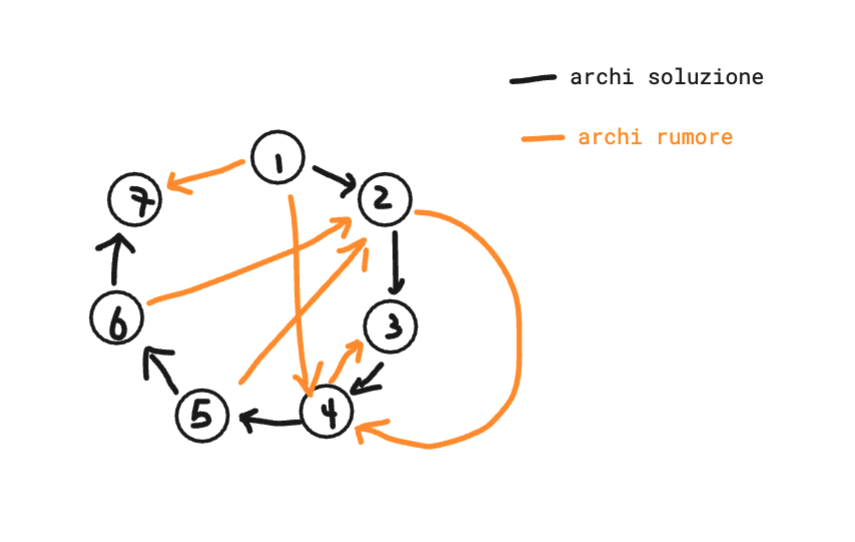
\includegraphics[width=0.7\linewidth]{img/hpp dna graph 1}
	\caption{Uno dei primi tentativi di istanze per HPP in DNA Computing.}
	\label{fig:1}
\end{figure}

\begin{enumerate}
\item Codificare i vertici (ed archi) nel DNA: una possibile codifica può essere la seguente: 
\begin{center}
\begin{tabular}{ c c c c c c c }
 $V_{1}$: & A & A & A & A & A & A \\ 
 $V_{2}$: & T & T & T & T & T & T \\
 $V_{4}$: & T & T & T & T & T & A
\end{tabular}
\end{center}
da notare che si sono scelti i vertici 1, 2 e 4 in quanto nel grafo $G$ vi è un arco da 1 a 2 e un arco da 1 a 4; una volta che si sceglie la codifica, queste sequenze vengono poste all'interno di una fiala, si otterrà quindi la seguente reazione a partire dalla tre sequenze iniziali (delle quali ricordiamo che abbiamo svariate copie):
\begin{itemize}
\item Si otterrà questa prima doppia sequenza:
\begin{center}
\begin{tabular}{ c c c c c c }
 A & A & A & A & A & A \\ 
 T & T & T & T & T & T \\
\end{tabular}
\end{center}
\item Si otterrà questa seconda doppia sequenza:
\begin{center}
\begin{tabular}{ c c c c c c c }
 A & A & A & A & A & A & X \\ 
 X & T & T & T & T & T & A
\end{tabular}
\end{center}
da notare che, in questo contesto, le X rappresentano degli spazi vuoti (sticky ends) e non una base azotata generica; da questo punto possiamo intuire che gli sticky ends possono essere utilizzati per rappresentare gli archi, quindi in una doppia sequenza siamo attualmente in grado di codificare sia i vertici che gli archi "di collegamento" tra essi.
\end{itemize}
\item Connettere i vertici tramite gli archi.
\item Filtrare le sequene risultanti in base alla lunghezza, infatti una soluzione esatta può essere tale solo se la lunghezza del path è pari alla lunghezza della "vera" soluzione, in questo caso la lunghezza della soluzione vera è 7, considerando che saranno necessari circa 10 basi azotate per rappresentare un vertice, significa che si filtrerà quindi si manterranno solo sequenze lunghe 70 basi azotate = 7 vertici * 10 $\dfrac{basi \quad azotate}{vertice}$; si noti che comunque controllare solo la lunghezza non garantisce di trovare una soluzione esatta, infatti si potrebbe essere incappati in un ciclo di lunghezza 7.
\end{enumerate}

Dato il grafo in figura \ref{fig:1} l'approccio di Adleman era il seguente:
\begin{enumerate}
\item Generare sequenze di DNA con path casuali, facendo in modo che l'HP venga rappresentato con una probabilità molto alta; da notare che la quantità di sequenze di DNA usate eccedeva di molto la quantità necessaria a rappresentare tutti i path del grafo scelto, così da fare in modo che molte delle sequenze rappresentassero con molte probabilità il HP.
\item Rimuovere tutte le sequenze che non codificano il HP.
\item Controllare che le sequenze rimanenti codificassero la soluzione per l'HPP.
\end{enumerate}
Adleman ha quindi implementato un algoritmo brute force per HPP tramite i seguenti step:
\begin{enumerate}
\item ogni vertice / arco veniva codificato tramite una sequenza distinta composta da 20 basi, questo significa che le sequenze contenenti il HP sono erano lunghe 20 * 7 = 140 basi; queste sequenze vengono poste nella fiala, quindi, una volta che iniziano a legarsi tra loro, si stima che si avranno una percentuale molto alta di sequenze che rappresentano un HP (non necessariamente quello esatto).
\item Quindi ha usato la PCR per aumentare di molto le sequenze che iniziano nel vertice 1 e terminano nel vertice 7, facendo in modo che esse siano la maggior parte di quelle presenti nella fiala; poi ha rimosso tutte quelle sequenze con lunghezza diversa da 140, per poi effettuare altri passaggi per mantenere solo le sequenze in cui tutti i vertici vengono attraversati una ed una sola volta.
\item In questo punto si riapplica la PCR, $n-1$ volte, dove $n$ è il numero di vertici del grafo in input (anche se non ho capito bene a che scopo).
\end{enumerate}

\section{SAT - Lipton}
Il lavoro di Lipton è fondamentale in quanto capisce che il lavoro di Adleman su HPP-DNA è rivoluzionario ma limitato ad usare il DNA Computing solo per risolvere HPP, Lipton vuole quindi trovare un modo per utilizzare il DNA Computing come modello formale di calcolo, ma non solo per HPP. Uno dei problemi in cui Lipton è incappato durante questo suo progetto è stato quello di dover rappresentare l'assegnamento di una formula booleana, per l'appunto l'input di SAT, tramite sequenze di DNA; la soluzione a cui è arrivato è la seguente: utilizzare dei grafi per rappresentare le sequenze di bit, più nello specifico, ogni vertice rappresenta una variabile, quindi si hanno due archi in uscita, che rappresentano il valore della variabile a $0$ o $1$, vedere figura \ref{fig:2}

\begin{figure}[h]
	\centering
	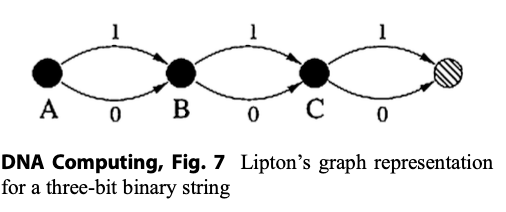
\includegraphics[width=0.5\linewidth]{img/lipton three bit}
	\caption{Questo grafo codifica una stringa di tre bit / variabili; grazie a questa rappresentazione, qualsiasi stringa di tre bit può essere rappresentata, infatti per ognuno dei bit / variabile si può scegliere se porla a $1$ path superiore oppure a $0$ path inferiore. In questo modo, Lipton ha riutilizzato il lavoro di Adleman "costruendoci" sopra. Da notare che vi è un nodo finale che non rappresenta alcuna variabile, è detto "dummy node" e serve solo per dare un nodo di arrivo ai vertici che escono "dall'ultima" variabile.}
	\label{fig:2}
\end{figure}
L'approccio di Lipton per risolvere SAT è stato quindi il seguente: grazie alla codifica appena descritta (in figura \ref{fig:2}) è necessaria una sola sequenza di DNA per vertice / arco, quindi, una volta che si mescolano le sequenze nella fiala, dei path random si andranno a formare spontaneamente; l'idea di Lipton era quindi quella di inserire nella fiala tutte le possibile stringhe (assegnamenti di verità) di una data lunghezza; si andrà quindi a rimuovere tutte le sequenze che non soddisfano la formula da risolvere; per fare ciò, si procede una clausola alla volta, rimuovendo tutte le sequenze che non la soddisfano, una volta fatto ciò, si procede con la clausola successiva, quindi si ripete il processo fino a che non vi sono più clausola da verificare; a questo punto, se sono rimaste delle sequenze, esse soddisfano la clausola.Insieme iniziale: "initial multi-set" è composto da stringhe di lunghezza $\bigcirc(n)$ dove $n$ è la dimensione del problema; questo multi-set dovrebbe contenere un sottoinsieme contenente tutte le possibili soluzioni (ognuna codificata sotto forma di stringa). Vediamo ora la schematizzazione dell'algoritmo di Lipton per SAT:
\begin{enumerate}
\item Costruire il set iniziale, detto $T$
\item For ogni clausola begin:
\begin{enumerate}
\item For ogni letterale $v_{i}$ begin:
\begin{enumerate}
\item If $v_{i} = x_{j}$ si estraggono da $T$ tutte le stringhe che hanno $v_{i} = 1$
\item Else si estraggono da $T$ tutte le stringhe con $v_{i} = 0$
\end{enumerate}
\item End for
\item Si costruisce un nuovo set T effettuando un merge di tutte le stringhe estratte
\end{enumerate}
\item End for
\item Se il set $T$ \textbf{non} è vuoto, allora la formula booleana $I$ è soddisfacibile.
\end{enumerate}

\begin{note}
La differenza fondamentale tra l'algoritmo di Adleman e quello di Lipton è la seguente: Adleman genera svariati path, ma essi vengono generati con probabilità diverse: i path che rappresentano una soluzione vengono generati con molte più probabilità rispetto agli altri; Lipton, d'altro canto, qualsiasi path viene generato con le stesse probabilità di qualsiasi altro path, andrà quindi a rimuovere quelli che non costituiscono una soluzione.
\end{note}

\paragraph{Da BF a grafo}
Prima di passare ad hairpins-DNA specifichiamo come sia possibile rappresentare una qualsiasi formula booleana (non solo quelle espresse in CNF) tramite un grafo: ad esempio, se si ha un la seguente formula booleana: $(P1) \vee (P2)$ può essere rppresentata sotto forma di grafo come mostrato in figura \ref{fig:3}; se avesse invece una formula booleana del tipo $(P1) \wedge (P2)$, la si può codificare in un grafo come mostrato in figura \ref{fig:4}; si noti che tutto ciò può essere espresso ricorsivamente, quindi, sia $P1$ che $P2$ possono avere all'interno, a loro volta, delle parti poste in and / or; questa parentesi è servita per mostrare che è possibile rappresentare sotto forma di grafo qualsiasi tpo di formula booleana, quindi si è ottenuto un "modello generico".
\begin{figure}[h]
	\centering
	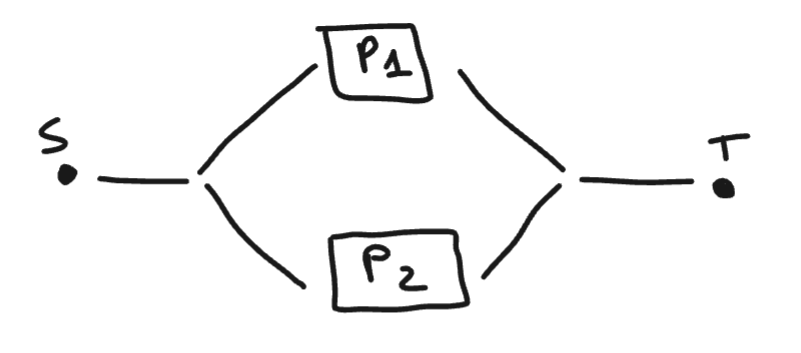
\includegraphics[width=0.5\linewidth]{img/bf to graph 1}
	\caption{Rappresentazione di una formula booleana, sotto forma di grafo, con due clausole in or tra loro.}
	\label{fig:3}
\end{figure}

\begin{figure}[h]
	\centering
	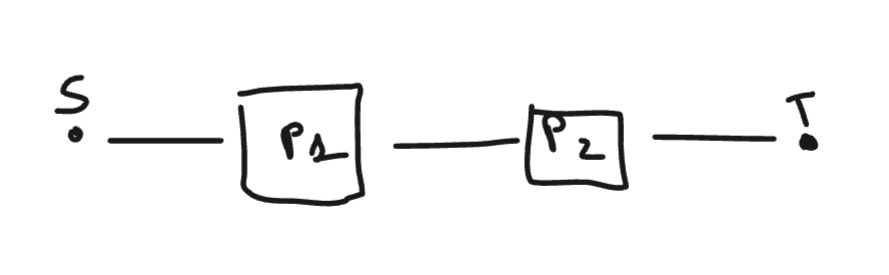
\includegraphics[width=0.5\linewidth]{img/bf to graph 2}
	\caption{Rappresentazione di una formula booleana, sotto forma di grafo, con due clausole in and tra loro.}
	\label{fig:4}
\end{figure}

\section{SAT - Hairpins}
Questa parte è dedicata ad una "sottoparte" del DNA Computing; hairpins DNA è DNA Computing con una caratteristica in più: gli hairpins (in italiano: forcine per capelli); sono delle strutture che si formano a partire da una sequenza signola di DNA, in quanto, la forza attrattiva che si erifica tra basi azotate complementari, avviene anche tra basi appartenenti alla stessa sequenza singola, si veda l'esempio \ref{eg - hairpins DNA}.

\begin{esempio}
\title{\emph{Hairpins in DNA}}
\label{eg - hairpins DNA}

A partire dalla seguente singola sequenza di DNA:
\begin{center}
\begin{tabular}{ c c c c c c c c c c c c c c}
 ... & X & X & A & A & X & X & X & X & T & T & X & X & ...
\end{tabular}
\end{center}
Una volta portata ad una certa temperatura, si avrà una reazione, che porterà ad ottenere la seguente sequenza:
\begin{center}
\begin{tabular}{ c c c c c c c c c }
 ... & X & X & A & A & X & X & $\rightarrow$ & $\downarrow$ \\
 ... & X & X & T & T & X & X & $\leftarrow$ & $\leftarrow$
\end{tabular}
\end{center}
Avremo quindi che, nel punto in cui avviene l'occorrenza delle due AA, fino a dove avviene l'occorrenza delle due TT, è una sezione considerata come doppia sequenza, il resto no (a meno che non vi siano altri hairpins).
Si noti che, in questo caso, le X rappresentano delle basi azotate che al momento non ci interessano.
\end{esempio}

Vediamo ora com'è possibile risolvere il problema SAT in \textbf{tempo costante} tramite l'aiuto del Hairpins-DNA Computing: l'approccio è molto diverso da quello di Lipton, infatti, in questo caso, non si vogliono generare tutte le possibili sequenze al principio della computazione oer poi andare a filtrarle, ma si vogliono costruire solo quelle che rappresentano una soluzione (queste potranno essere di due tipi: legali e non-legali); per generare quindi tutte e sole le sequenze che soddisfano la formula booleana hairpins-DNA usa la seguente strategia:
\begin{enumerate}
\item Per ogni clausola si sceglie un letterale e lo si soddisfa.
\item Il punto 1) è ripetuto per tutte le clausole, ma non solo, è ripetuto anche fino a che si sono ottenute tutte le singole sequenze composte dalle combinazioni di letterali scelti all'interno di una singola clausola.
\item Una volta fatto ciò, si avranno tutte le soluzioni, sia legali che non quelle non legali sono quelle con almeno un hairpins (ciò significa che per soddisfare la formula booleana si è posto uno stesso letterale sia a true che a false, cosa che ovviamente non è "legale").
\item Si andrà quindi a rimuovere tutti gli hairpins da tutte le sequenze che ne contengono uno o più.
\item Quindi, se la soluzione, meno gli hairpins, è ancora di una certa lunghezza (vedi nota \ref{nota - lunghezza della soluzione}), allora si è trovata la soluzione.
\end{enumerate}

\begin{note}
\title{\emph{Lunghezza della soluzione}}
\label{nota - lunghezza della soluzione}

Una volta rimossi tutti gli hairpins, per verificare se la sequenza ottenuta è una soluzione oppure no, si controlla se la lunghezza della sequenza è pari a: numero di clausole(ad esempio 10) * n° di basi azotate per rappresentare una variabile(ad esempio 4) = 40; quindi se la sequenza che si sta controllando è di lunghezza 40, essa è una soluzione.
\end{note}

\begin{note}
\title{\emph{Considerazioni sul tempo}}
Vediamo ora com'è possibile che questo tipo di computazione avvenga in tempo costante, possiamo semplificare la computazione in tre step:
\begin{enumerate}
\item Generare le sequenze: questo step richiede tempo costante in quanto avviene in parallelo, quindi richiede sempre lo stesso tempo indipendentemente dalla dimensione dell'input, richiede quindi $\bigcirc(1)$.
\item Lasciare che si formino gli hairpins: si applica lo stesso ragionamento del punto 1, quindi si ha tempo $\bigcirc(1)$.
\item Rimuovere gli hairpins dalle sequenze che ne contengono: si applica lo stesso ragionamento del punto 1, quindi si ha tempo $\bigcirc(1)$.
\end{enumerate}
\end{note}

\begin{note}
\title{\emph{Svantaggi del Hairpins DNA}}

Il punto che rende svantaggioso hairpins DNA è che richiede un numero di sequenze maggiore rispetto a Lipton, quindi il numero di errori aumenta a sua volta (se migliora il tempo, di solito peggiora qualcos'altro); più nello specifico:
\begin{itemize}
\item Lipton: $ \sim 2^{n}$ sequenze richieste.
\item Hairpins DNA: $ \sim 3^{4*n}$ sequenze richieste.
\end{itemize}
\end{note}

\chapter{Cellular computing}
\begin{figure}[h]
	\centering
	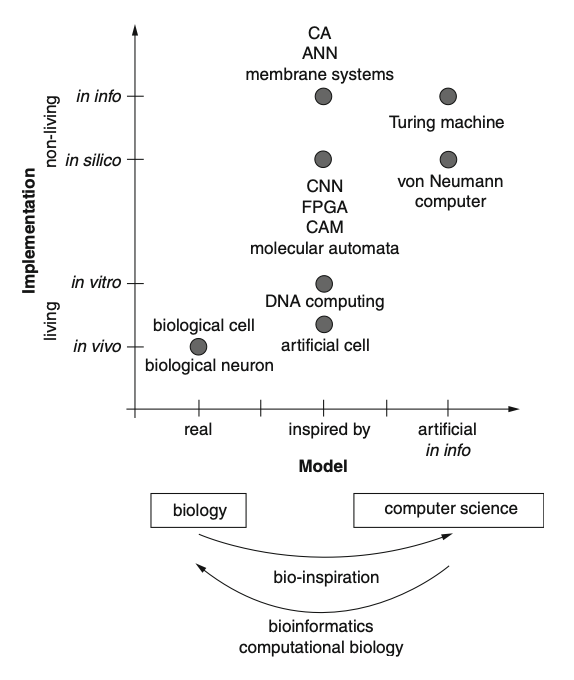
\includegraphics[width=0.7\linewidth]{img/cellular computing}
	\caption{Illustration of the various possibilities to implement cellular models that range from realistic to abstract. Drawing inspiration from biology to build better computing machines is known under the term bioinspiration, while using machines to address problems in biology is known as bioinformatics and computational biology}
	\label{fig:5}
\end{figure}
In 1999, Moshe Sipper, used the term “cellular computing” in a broad sense to introduce a general computing philosophy and framework. He hypothesized that Cellular computing consists of three essential and admittedly very general principles:
\begin{itemize}
\item \textbf{Semplicità}: i singoli elementi sono di carattere semplice, ma, nel complesso, possono portare a risultati molto complessi: ottenere un "global behavior" a partire da tante "local interactions".
\item \textbf{Vasto Parallelismo}: tipicamente i singoli elementi lavorano in parallelo, portando a risultati locali che verrà poi condivisi con il resto del sistema.
\item \textbf{Località}: il sistema viene descritto come l'aggregazione di elementi semplici che calcolano e si scambiano i vari risultati locali (con i quali si può poi continuare nella computazione).
\end{itemize}
Oltre ai tre principi fondamentali enunciati da Sipper, ci sono altri parametri da considerare nel Cellular computing:

\paragraph{Struttura topologica}
considerare la struttura topologica dei singoli elementi che vanno a comporre
l'insieme, si possono avere diversi modelli: uniformi, non uniformi, uniformi e composti da singoli elementi tutti uguali, non uniformi e composti da singoli elementi che possono anche essere di diversi tipi ecc. (vedi figura \ref{fig:cell-comp-topo}); oltre a ciò è possibile che un singolo elemento sia a sua volta formato da altri elementi singoli (una sorta di induzione), che a loro volta possono essere tra loro dello stesso tipo, diversi, uniformi o non; tutte queste possibilità portano ad un evoluzione della computazione che, anche a parità di input nei vari singoli elementi, porta invece ad un risultato molto diverso, tra i vari singoli elementi, al termine dello step di computazione.

\paragraph{Interconnessione}
da considerare anche l'interconnessione tra i singoli elementi, altro aspetto particolare in quanto i vari elementi non sanno se sono connessi o meno ad altri elementi, sanno solo che producono un risultato e poi lo mandano in output.
\begin{figure}[h]
	\centering
	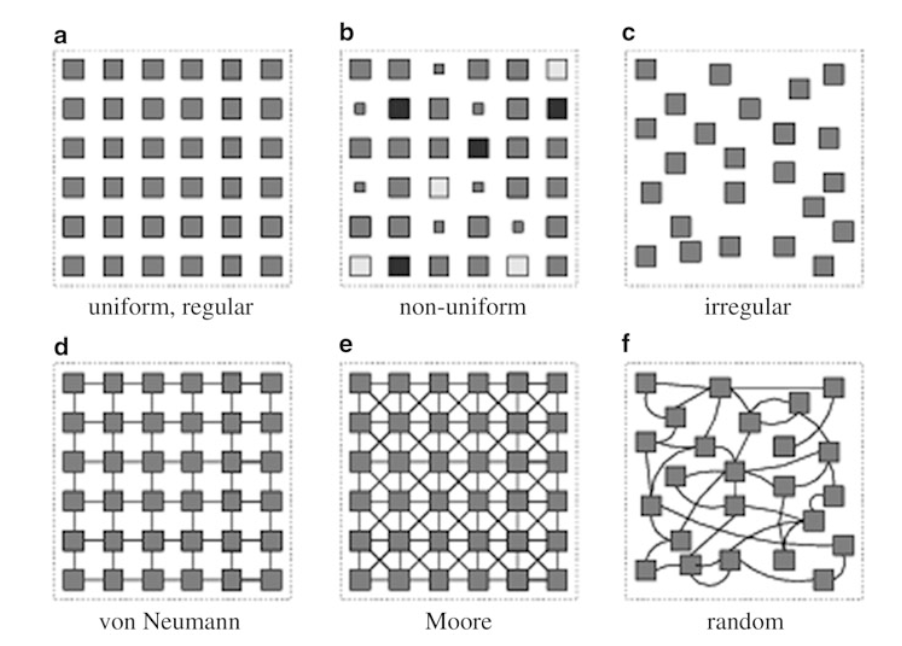
\includegraphics[width=0.5\linewidth]{img/celllular computing topology}
	\caption{Illustration of different cell arrangements and interconnect topologies. (a) Regular and uniform; (b) regular and nonuniform, different shadings and sizes indicate different cell programs; (c) irregular and
uniform; (d) regular, uniform, von Neumann neighbor- hood; (e) regular, uniform, Moore neighborhood; (f) irreg- ular, uniform, random neighborhood}
	\label{fig:cell-comp-topo}
\end{figure}
I modelli principali di cellular computing sono i seguenti: Cellular Automata, Membrane Computing, Amorphous Computing; a seconda del modello che si sta studiando, bisogna effettuare le dovute considerazioni sull'hardware con il quale lo si vuole implementare; tre aspetti da considerare, quando si implementa uno di questi modelli, sono i seguenti: computabilità, efficienza e affidabilità.

\section{Cellular Automata} Because in this course we have never saw cellular automata before, we will now do an easy introduction: it consider a discrete space, than split it in multiple cells, each cell has a value that can evolve for every iteration, typically the new value of a cell is related to the old value of that same cell and also to the value of some neighbourhood cells (that may be all, more or just a few of the neighbourhood); the values that a cell can assume are base on $N$ states; this formalism implement max parallelism, in fact,  for every iteration, the whole systems state change; note that, also in this type of formalism, the memory and processor overlap, in fact the computation depend also on the value of a single cell, and the computation also happens in the cell. A cellular automata $A$ will be described as follow: $ A = (S, Q, N, R) $ where:
\begin{itemize}
\item $S$ is the space, typically 1D - 2D (but can also be 3D, 4D, 5D).
\item $Q$ is the set of states that every cell can assume during the computation.
\item $N$ is the definition of the neighbourhood, let's see two of the most used neighbourhoods:
\begin{itemize}
\item Von Neumann neighbourhood: see figure \ref{VN - neighbourhood}, this neighbourhood can be described in terms of coordinate as follow: $$ N^{VN} = \lbrace (x, y) : |x - x_{i}| + |y - y_{i}| \leq 1 \rbrace $$
\item Moore neighbourhood:  see figure \ref{M - neighbourhood}, this neighbourhood can be described in terms of coordinate as follow: $$ N^{M} = \lbrace (x, y) : |x - x_{i}| \leq 1 \wedge |y - y_{i}| \leq 1 \rbrace $$
\end{itemize}
Note that not every cell has a whole neighbourhood, in fact, boundaries cells have not a whole neighbourhood; to solve this problem there are two ways: virtual neighbourhood or considering choroid form space.
\item $R$ is the rewriting rule.
\end{itemize}
\begin{figure}[h]
	\centering
	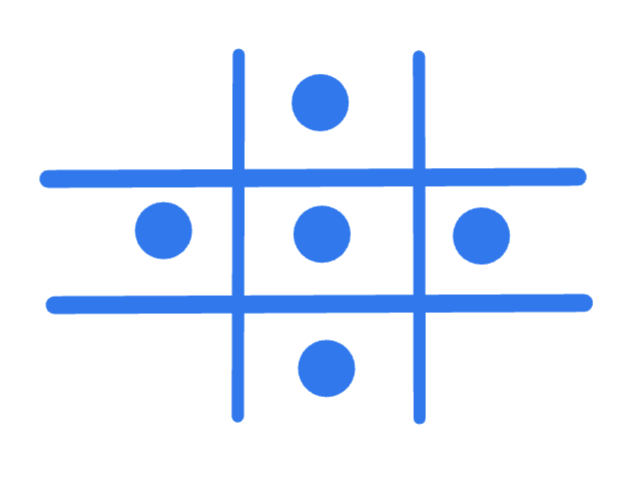
\includegraphics[width=0.3\linewidth]{img/VN - neighbourhood}
	\caption{Von Neumann neighbourhood representation.}
	\label{VN - neighbourhood}
\end{figure}
\begin{figure}[h]
	\centering
	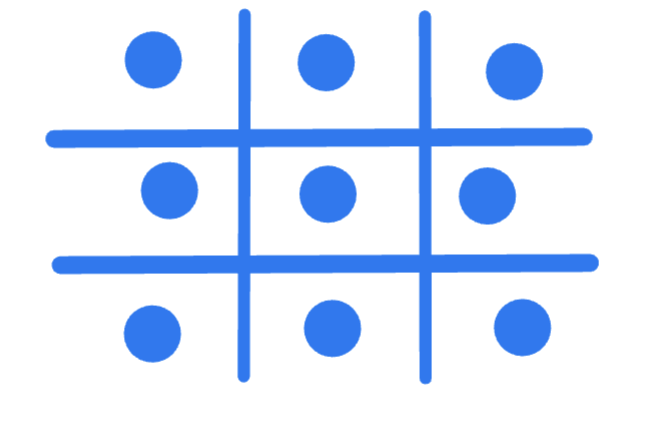
\includegraphics[width=0.3\linewidth]{img/M - neighbourhood}
	\caption{Moore neighbourhood representation.}
	\label{M - neighbourhood}
\end{figure}

\section{Membrane systems}
\label{membrane systems}
Questi sistemi sono chiamati così proprio perché la membrana è uno dei suoi elementi principali; uno degli intenti principali nello sviluppo di questi sistemi è di \textbf{investigare le proprietà computazionali della cellula}, di poter confrontare ciò con altri modelli (TM, CA, ecc...); studiare possibili applicazioni a problemi computazionali / biologici. Questo modello è stato inventato nel 1998, ed è ispirato alla struttura ed al funzionamento della cellula; è un modello discreto: si ha una quantità fissa di elementi chimici e delle possibili reazioni tra queste sostanze. Vediamo ora alcune caratteristiche dei sistemi a membrana (queste caratteristiche vengono ereditate dal cellular computing):

\subparagraph{Discreto}
come già spiegato in precedenza, si hanno una quantità fissa di elementi chimici e delle possibili reazioni tra queste sostanze.

\subparagraph{Parallelismo massimo}
tutte le sotto parti eseguono e scambiano operazioni contemporaneamente; questo parallelismo avviene anche a livello del singolo elemento, nel senso che se in un singolo elemento della struttura vi sono tre sostanze chimiche, allora la reazione avviene in parallelo su tutte e tre, e non in maniera sequenziale; possiamo quindi dire che c'è una sorta di "doppio parallelismo" ossia uno a livello globale ed un altro a livello dei singoli elementi.

\subparagraph{Non determinismo}
tipicamente non si ha determinismo, ciò dipende dalle regole usate, ad esempio una sostanza chimica $A$, dopo una reazione diventa $B$, ma potrebbe anche diventare $C$; si hanno quindi due modelli diversi: confluent / non-confluent; se il sistema considerato è confluent significa che il risultato finale sarà lo stesso per tutte le computazioni, ma le computazioni intermedie possono risultare diverse tra loro; se invece si considera un sistema non-confluent, significa che a livello intermedio si possono avere computazioni che risultano diverse tra loro (path differenti) ma non solo, anche il risultato finale potrebbe essere diverso tra le varie computazioni (ossia vero non determinismo). Ovviamente è possibile anche realizzare questo modello con delle regole deterministiche.

\paragraph{Componenti}
vediamo ora quali sono i componenti dei sistemi a membrana, questi componenti sono delle astrazioni della reale struttura della cellula:

\subparagraph{Membrane}
tutto ciò che svolge la funzione di confine, ossia definisce l'interno dall'esterno della cellula; questi confini, a livello interno della cellula, si chiamano \textit{regioni}; queste membrane si distinguono in elementari e non-elementari; le membrane elementari non contengono altre membrane (ma possono contenere altre strutture); le membrane non-elementari contengono una o più altre membrane. La membrane principale, più esterna, è detta \textit{skin}.

\subparagraph{Sostanze chimiche}
l'astrazione di questo elemento sono \textbf{multiset di simboli} o \textbf{stringhe}; si ricorda che un multiset è un set nel quale si tiene conto di quante "istanze" vi sono di un certo elemento.

\subparagraph{Reazioni}
le reazioni chimiche vengono implementate tramite delle \textit{regole di riscrittura}, vediamone alcune:
\begin{itemize}
\item $a \rightarrow xy$ \textbf{regola non cooperativa}: queste regola prende un simbolo e lo trasforma in un multi-set di simboli, senza considerare il "contesto" del simbolo iniziale.
\item $ab \rightarrow xy$ \textbf{regola cooperativa}: questa regola, a differenza della prima, conosce il "contesto"  del simbolo, quindi, in questo caso specifico, la reazione avviene se e solo se è presente sia l'elemento $a$ che l'elemento $b$ (più potente rispetto alla precedente).
\item $ac \rightarrow xc$ \textbf{regola catalitica}: conosce il contesto, ma non consuma la "parte catalitica" infatti l'elemento $c$ non viene consumato (ha una potenza intermedia rispetto le due regole precedenti).
\end{itemize}

\subparagraph{Regole di comunicazione}
i risultati si possono comunicare tramite le regioni, nello specifico vengono comunicati ad una regione vicina:
\begin{itemize}
\item \textbf{Here}: mantenere il risultato nella regione in cui è avvenuta la reazione.
\item \textbf{Out}: ossia mandare il risultato all'esterno rispetto la membrana in cui è avvenuta la reazione.
\item \textbf{In}: mandare il risultato in una delle strutture contenute rispetto a dove è avvenuta la reazione; in questo caso, se all'interno della struttura è presente più di una sotto-struttura, allora sarà necessario effettuare una scelta.
\end{itemize}
Per realizzare questo scambio, tipicamente si applicano delle etichette alle membrane, così è possibile specificare a che membrana si vuole mandare il risultato. tipicamente il labelling segue questo scehma: alla membrana skin viene associata l'etichetta 0, alla prima membrana più interna 1 ecc... .

\subparagraph{Eliminazione}
operazione che consiste nell'eliminare la membrana  una volta che il risultato è stato comunicato al target; in gergo si dice che la membrana "viene aperta";
quest'operazione viene indicata ponendo il simbolo $\delta$ al termine della regola di comunicazione (si noti che questa operazione non può essere applicata alla skin-membrane, infatti la skin.membrane non può essere distrutta).

\subparagraph{Priorità tra regole}
è da considerare anche la priorità tra regole che rendono possibili i vari path, infatti, le regole vengono applicate in ordine di priorità, una regola può essere applicata solo se non vi sono altre regole di priorità maggiore che possono essere applicate in quel dato momento; se vi sono più regole che possono essere eseguite nello stesso momento, allora si segue una scelta non-deterministica.

\begin{esempio}
\title{\emph{Comunicazione delle reazioni}}
\begin{itemize}
\item $a \rightarrow (x, here) (y, out) (z, in_{3})$: questo esempio di comunicazione indica che si hanno tre elementi come risultati: $x, y, z$, e vengono mandati rispettivamente:
\begin{itemize}
\item Rimane nella stessa regione.
\item Viene mandato all'esterno.
\item Viene mandato all'interno, nello specifico nella membrana con etichetta $3$.
\end{itemize}
\end{itemize}
\end{esempio}

\begin{definizione}
\title{\emph{Membrane system}}

$\Pi = (V, \mu, M_{1}, ..., M_{n}, (R_{1}, \rho_{1}), (R_{n}, \rho_{n}), i_{0})$
dove:
\begin{itemize}
\item $V$: alfabeto
\item $\mu$: rappresenta la struttura della membrana (Ex. $[ \quad [ ]_{2} [ ]_{3} \quad [ \quad [ ]_{5} [ ]_{6} \quad ]_{4} \quad ]_{1}$).
\item $M_{i}$: è il multiset dei simboli / stringhe in $V$.
\item $R_{i}$: è l'insieme finito delle regole di evoluzione
$x \rightarrow y, x \in V^{+}, y = y^{'}$ or $y = y^{'} \delta $
\item $\rho_{1}$: è l'ordine parziale delle relazioni tra $R_{i}$.
\item $i_{0}$: è la membrana output; se vuota allora si considera l'ambiente come regione output.
\end{itemize}
\end{definizione}

\paragraph{Aspetti computazionali}
Enunciamo alcuni apsetti computazionali importanti dei sistemi a membrana:
\begin{enumerate}
\item $NOP_* (coo, tar) = NOP_1 (coo, tar) = NRE$
ossia: la famiglia di numeri naturali generati da un P system senza limitazioni sul numero di membrane che utilizza (*), e che ha a disposizione la regola cooperativa ed il target, è uguale alla famiglia di numeri naturali generati dal P system che utilizza una sola membrana e che ha a disposizione la regola cooperativa ed il target, che è a sua volta uguale alla famiglia dei linguaggi ricorsivamente enumerabili.
\item $NOP_* (ncoo, tar) = NOP_1 (ncoo, tar) = CF$
ossia: la famiglia di numeri naturali generati da un P system senza limitazioni sul numero di membrane che utilizza (*), e che ha a disposizione la regola non-cooperativa ed il target, è uguale alla famiglia di numeri naturali generati dal P system che utilizza una sola membrana e che ha a disposizione la regola non-cooperativa ed il target, che è a sua volta uguale alla famiglia dei linguaggi context-free.
\item $NOP_* (ncoo, tar) \subset NOP_2(NCOO, tar, \delta)$
ossia: la regola di dissoluzione aumenta la potenza computazionale.
\end{enumerate}

Vediamo quindi ora come avviene il processo di computazione nel calcolo a membrana:
\begin{definizione}
\title{\emph{Computazione / evoluzione nei sistemi a membrana}}
\begin{itemize}
\item $M_{1}, ..., M_{n}$ configurazione iniziale.
\item Vengono applicate le regole secondo le priorità.
\item Vengono applicate le regole secondo il non determinismo.
\item Tutti gli oggetti e tutte le regioni evolvono in parallelo.
\item Le regole possono muovere gli oggetti tra le membrane.
\item La membrana viene dissolta ($\delta$).
\end{itemize}
\end{definizione}

\paragraph{Altre features}
in questa sezione abbiamo visto che solo alcune delle caratteristiche della cellula sono state "implementate" nel sistemi a membrana, questo non significa che non se ne possano considerare altre; ad esempio gli inibitori o i promotori, i primi fanno in modo che una regola possa essere applicata sse il multiset iniziale non contiene un certo simbolo, i secondi fanno il contrario. Si può anche andare a considerare lo spessore di una membrana, quindi andare a cambiarla, fino a renderla impermeabile oppure a distruggerla ($\delta$). È anche possibile cambiare il funzionamento dello scambio di oggetti di una membrana, ad esempio mandando due oggetti nei due versi opposti (uniport, symport, antiport).

\subsection{Sistemi a membrana attiva}
Nel modello generale dei sistemi a membranam, la membrana non ha un ruolo attivo nello scambio di oggetti. Questo modello considera invece delle membrane attive, sia a livello di comunicazione che a livello di processo, questo significa che anche le regole di comunicazione / evoluzione sono diverse, in quanto devono tenere in considerazione l'attuale carica associata alla membrana in cui sta avvenendo la reazione.
\paragraph{Labelling}
nei sistemi a membrana attiva, rispetto ai sistemi a membrana classici, al posto delle label $(1, 2, 3, ..., n)$ per identificare la membrana target di una regola di comunicazione, si utilizza la polarizzazione elettrica $(+, -, 0)$, quindi non si potranno sempre identificare univocamente tutte le mebrane, sarà invece più probabile che vengano separate in gruppi (e.g.: tutte quelle a carica positiva o tutte quelle a carica negativa).

\paragraph{Division rule}
uno degli aspetti più importanti dei sistemi a membrana attiva è l'implementazione di una caratteristica fondamentale della cellula, ossia la divisione di se stessa:
\begin{itemize}
\item Elementary division: divisione di un oggetto elementare.
\item Non-elementary division: divisione di un oggetto non elementare, vengono duplicate quelle membrane che hanno polarizzazione neutrale.
\end{itemize}
Questa caratterstica è fondamentale, proprio perché, se sfruttata correttamente, ha la potenzialità di avere un numero esponenziale di processori rispetto al tempo di esecuzione.

\paragraph{One rule at each step}
Un'altra differenza tra i sistemi a membrana classici e quelli a membrana attiva sta nel fatto che ad ogni step, ad una determinata membrana si può applicare una singola regola, e non più di una (e.g.: esempio non si può comunicare in due sensi e duplicare la membrana contemoraneamente: o si applica un'operazione, oppure l'altra).

\subsubsection{SAT}
\label{SAT - Linear time}
Tramite i sistemi a membrana attiva è possibile risolvere SAT in tempo lineare, è infatti possibile generare tutti i possibili assegnamenti di verità in $n$ step di computazione, vedi esempio \ref{ex - lin time sat 1}, dopo ciò è possibile far passare la polarizzazione di ogni membrana da neutra a positiva, si fa ciò trasportando all'esterno i vari $z_{n}$, quindi, tutti i $T_{i}$ vengono rimpiazzati da $R_{h_{i}}$ dove $h_{i}$ è l'indice di una clausola che viene soddisfatta proprio dall'assegnamento $T_{i}$; a questo punto è necessario controllare solo se esiste una membrana che contiene tutti i $R_{h_i}$; per fare ciò bastano $2*m$ passi di computazione; quindi, \textbf{per riassumere}: si parte con una configurazione iniziale, dopo esattamente $n+2m+2$ step di computazione si controlla se si ha una $T$ (nella membrana skin), allora la risposta è SI, se non vi è una $T$ allora la risposta è NO; si noti quindi che il tempo è polinomiale ma lo spazio è esponenziale.
\begin{note}
Un'altra nota da fare è che con input diverse sarà necessario avere delle regole diverse, questa caratteristica è detta "soluzione semi uniforme".
\end{note}


\begin{esempio}
\title{\emph{linear time SAT}}
\label{ex - lin time sat 1}

Considerando la seguente configurazione iniziale:
$$[ \quad [z_{1} \quad a_{1} a_{2} ... a_{n}]_{2}^{0} \quad ]_{1}^{0}$$
si vuole poter considerare ogni possibile assegnamento di verità, per fare ciò, si parte dal primo letterale $a_{1}$ e lo si assegna a true $(T_{1})$ nella prima copia ed a false nella seconda copia $(F_{1})$ , utilizzando la division rule, come segue:
$$[ \quad [z_{2} \quad T_{1} \quad a_{2} ... a_{n}]_{2}^{0} \quad [z_{2} \quad F_{1} \quad a_{2} ... a_{n}]_{2}^{0} \quad ]_{1}^{0}$$
ripetendo il suddetto processo per n (possibile contare il numero di step tramite l'elemento $z_{n}$) volte si otterranno quindi tutti i possibili assegnamenti di verità.
Si cambia quindi la polarizzazione di tutte le membrane da neutra a positiva trasportando $z_{n}$ all'esterno:
$$[ \quad [T_{1} \quad T_{2} ... T_{n}]_{2}^{+} \quad [T_{1} \quad T_{2} ... T_{n-1} \quad F_{n}]_{2}^{+} \quad ... \quad [F_{1} \quad F_{2} ... F_{n}]_{2}^{+} \quad ]_{1}^{0}$$
\end{esempio}

\subsection{Recognizer P systems}
I recognizer P system, tipicamente indicati con $\Pi$, sono quei sistemi nei quali, al termine della computazione, si va a verificare il contenuto della skin membrane
\begin{note}
In questi sistemi, al termine della computazione la skin membrane potrà contenere solo YES oppure NO
\end{note}
Ovviamente se si ha YES nella skin membrane significa che la computazione è stata accettata, altrimenti rifiutata.

Facciamo ora chiarezza sulle classi di complessità in questo ambito:
\begin{definizione}
\title{\emph{Classi computazionali}}
\begin{itemize}
\item $MC_{T}(f)$ è l'insieme dei linguaggi decisi da una famiglia semi-uniforme di P systems confluenti.
\item $PMC_{T}(f)$ è l'insieme dei linguaggi decisi, in tempo polinomiale, da un P system confluente, dove $T$ è una classe di recognizer P system.
\item $NMC_{T}(f)$ è l'insieme dei linguaggi decisi da una famiglia semi-uniforme di P systems non-confluenti.
\item $NPMC_{T}(f)$ è l'insieme dei linguaggi decisi, in tempo polinomiale, da una famiglia semi-uniforme di P systems non-confluenti.
\end{itemize}
\end{definizione}

Vediamo ora alcune delle classi ($T$) dei recognizer P systems:
\begin{itemize}
\item $AM$: sono quei recognizer P systems con membrana attiva tali che sono in grado di effettuare la divisione sia di membrane elementari che di non-elementari.
\item $\varepsilon AM$: sono quei recognizer P systems con membrana attiva tali che sono in grado di effettuare la divisione solo di membrane elementari.
\item $N AM$: sono quei recognizer P systems con membrana attiva; questa classe non è in grado di effettuare alcuna divisione.
\end{itemize}

Ora che abbiamo enunciato un po' di definizioni, possiamo analizzare alcune proprietà / relazioni tra questi sistemi:
\begin{itemize}
\item $ MC_{T}(f) \subseteq NMC_{T}(f) $, nello specifico si ha che: $ PMC_{T}(f) \subseteq PNMC_{T}(f) $.
\item $ MC_{N AM}(f) \subseteq MC_{\varepsilon AM}(f) \subseteq MC_{AM}(f) $
\item $ PMC_{N AM}(f) \subseteq PMC_{\varepsilon AM}(f) \subseteq PMC_{AM}(f) $
\item $ NPMC_{N AM}(f) \subseteq NPMC_{\varepsilon AM}(f) \subseteq NPMC_{AM}(f) $
\end{itemize}

\begin{definizione}
\title{$P = PMC_{N AM}$}
\label{P = PNC}

Siccome una TM deterministica è in grado di simulare un sistema confluente P , non in grado di effettuare divisioni, con i due seguenti step:
\begin{itemize}
\item Tenendo traccia del numero di elementi in ogni membrana.
\item Effettuando una simulazione della computazione del sistema P, simulando una regola della somma.
\end{itemize}

È quindi possibile affermare che $P = PMC_{N AM}$; si noti che la computazione della TM richiederà $n^{2}$ step di computazione, se si sta simulando un sistema $PMC_{N AM}$ che effettua $n$ step, è quindi polinomiale.
\end{definizione}

\begin{definizione}
\title{$NP = NPMC_{N AM}$}

Il ragionamento è diverso rispetto a quello della definizione \ref{P = PNC}, ma si arriva allo stesso risultato: $NP = NPMC_{N AM}$.
\end{definizione}

\pagebreak
\section{SNPS}

\paragraph{Introduction}
Si noti che questi sistemi possono essere usati per diverse applicazioni (e.g. problemi di classificazione nonché altri problemi complessi), noi andremo a vedere nello specifico come utilizzare questi sistemi per risolvere problemi NP completi (gli SN P systems considerati sono non deterministici "non-confluenti", infatti, è dimostrabile che gli SN P systems confluenti sono equivalenti ad una TM deterministica, e sono quindi meno potenti degli SN P non-confluenti, a meno che P=NP). A volte si fa riferimento a questi sistemi come il 3° tipo di reti neurali; Questi sistemi collegano concetti presi da più ambiti, tra cui  spiking systems e membrane systems (in this field it is normal that, a model is created taking inspirations from many other fields / models).

\paragraph{Energy Efficiency Considerations}
Possiamo affermare che i SN P systems richiedano meno energia nei due seguenti aspetti:
\begin{enumerate}
\item Serve meno training in confronto alle reti neurali.
\item Esiste hardware specifico, per implementare il modello discusso, che richiede meno energia per effettuare la computazione.
\end{enumerate}
Questi sistemi sono ispirati al funzionamento del neurone (che ricordiamo codificano informazioni sotto forma di cariche elettriche dette spikes, quindi, una volta raggiunta una certa soglia, comunicano il proprio messaggio ad altri neuroni, tramite le sinapsi, da questo deriva il nome).

\paragraph{Composition Elements}
Vediamo ora, più nello specifico, gli elementi che compongono gli SN P systems:
\begin{enumerate}
\item I neuroni: che possono essere associati ai vertici di un grafo diretto; ogni neurone è composto da un certo numero di spikes e da delle regole.
\item Firing Rule: (che comunica gli spikes agli tutti i neuroni connessi al neurone sorgente); nel momento in cui si esegue la firing rule, il neurone sorgente diventa chiuso per un certo periodo di tempo (detto \textit{delay}), se un neurone riceve una comunicazione mentre è in delay, allora la comunicazione viene semplicemente persa.
\item Forgetting Rule: (una volta raggiunto un certo numero spikes, allora li si può eliminare con questa regola), il controllo sul numero di spikes presenti viene effettuato confrontando gli spikes presenti con una certa \textbf{espressione regolare}; le forgetting rules possono essere applicate solo quando entrambe le seguenti condizioni sono soddisfatte:
\begin{enumerate}
\item Se nessuna firing rule può essere applicata.
\item Se si hanno esattamente $s$ spikes.
\end{enumerate}
Ad ogni unità di tempo, se vi è una regola che può essere applicata, allora viene applicata; se vi sono due o più regole che possono essere applicate nella stessa unità di tempo, allora una delle due viene scelta, non deterministicamente, per essere eseguita.
\item Synapse: le sinapsi sono il collegamento tra i vari neuroni.
\end{enumerate}

\paragraph{Computation}
A computation in terms of SN P systems is described as follow:
\begin{itemize}
\item Initial configuration: $n_{1}, n_{2}, ..., n_{m}$ are the spikes present in each neuron.
\item At the start all neurons are open.
\item During the computation the number of spikes in each neuron and the delay time of each neuron are tracked.
\item The real computation happens here: among configurations dictated by the rules.
\item Output: the output is represented by the time elapsed between the arrival of two different spikes in a designated output neuron.
\item If no input neuron is specified then use generative mode.
\item If no output neuron is specified then use accepting mode: accepts the numbers if the computations halt.
\item \textbf{Note}: a computation may not halt. 
\end{itemize}


\subsection{Subset sum}
\label{subset sum solution}
\paragraph{Instance}
Subset sum is a problem with two inputs:
\begin{itemize}
\item The first is a multi set $ V = \lbrace v_{1}, v_{2}, ..., v_{n} \rbrace $ where for all $i \in 1,...,n \quad v_{i} \in \mathbb{N}$.
\item The second input is a positive integer number $S$.
\end{itemize}
\paragraph{Output}
The output of the problem is whether or not exist a sub multi set $B \subseteq V$ such that $\displaystyle\sum_{b \in B} b = S$
\paragraph{Non Deterministic Solution}
Considering an instance if subset sum: $ (V = \lbrace v_{1}, v_{2}, ..., v_{n} \rbrace, S) $ our algorithm will make these steps:
\begin{itemize}
\item \textbf{Initial configuration}: the leftmost neurons will respectively contains $v_{1}, v_{2}, ..., v_{n}$ spikes; the rightmost neurons contain zero spikes.
\item \textbf{First step}: each leftmost neurons non deterministically decide if the element $v_{i}$ is to be included or not in the candidate solution $B \subseteq V$.
\item \textbf{Spikes happens}: a number of spikes equal to $N = |B|$ (corresponding to the sum of the $v_{i}$ that have been chosen) occurs in the right most neurons.
\item We now have three possible \textbf{cases}:
\begin{enumerate}
\item $ N < S $
\item $ N = S $
\item $ N > S $
\end{enumerate}
\item \textbf{Output}: The instance is positive if and only if a single spike is emitted.
\end{itemize}
\paragraph{Considerations}
We have seen how to solve subset sum in a non deterministic way, in a constant time and with a semi-uniform solution; can we now think about a way to implement a uniform solution for complex problems (such as SAT)? the answer is yes, and we will see how in section \ref{SAT solution}.

\subsection{SAT}
\label{SAT solution}
Al termine della sezione \ref{subset sum solution} abbiamo ribadito come la soluzione ottenuta fosse semi-uniforme, vediamo ora invece come risolvere un altro problema (SAT) tramite una soluzione uniforme.
Ricordiamo che per ottenere una soluzione uniforme dobbiamo rispettare due step:
\begin{itemize}
\item Descrivere il sistema.
\item Descrivere come si codifica la formula booleana in input.
\end{itemize}

\paragraph{Relation Between Variables And Clauses}
\label{Relation Between Variables And Clauses}
Vediamo quindi come esprimere la relazione tra variabile/letterale e clausola; possiamo affermare che esistono tre relazioni tra variabile e clausola:
\begin{enumerate}
\item La variabile non appare all'interno della clausola; possiamo pensare di codificare questa situazione come due bit a zero: $00$.
\item La variabile appare (in maniera diretta) all'interno della clausola; possiamo pensare di codificare questa situazione come due bit: il primo posto a zero, il secondo posto a uno: $01$.
\item La variabile appare (negata) all'interno della clausola; possiamo pensare di codificare questa situazione come due bit: entrambi posti a uno: $11$.
\end{enumerate}
La codifica sopra espressa può essere quindi espressa sotto forma di SN P system come segue:
\begin{itemize}
\item Zero spikes corrispondono a $00$.
\item Uno spike corrisponde a $01$.
\item Due spikes corrispondono a $11$.
\end{itemize}

\paragraph{Input Encoding}
Vediamo quindi come viene generato l'input per il resto del problema:
\begin{itemize}
\item Considerando un istanza di SAT con $m$ clausole e $n$ variabili:
\item Si avrà un neurone per ogni clausola: $m$ neuroni totali.
\item Si considerano tutte le clausole, quindi, per ogni variabile, si indica la relazione con tutte le clausole (in parallelo), quindi, siccome abbiamo $n$ variabile, questo step richiede almeno $n$ operazioni, ma siccome per ogni variabile sono necessari 2 spikes, allora in realtà questa operazione richiede $2n$ operazioni; questa operazione è detta di \textit{spike train} (vedi esempio \ref{sn p sol 1}), si ha quindi uno spike train per ogni clausola.
\item Introdurre l'input richiede quindi $2n$ passi.
\end{itemize}
\begin{figure}[h]
	\centering
	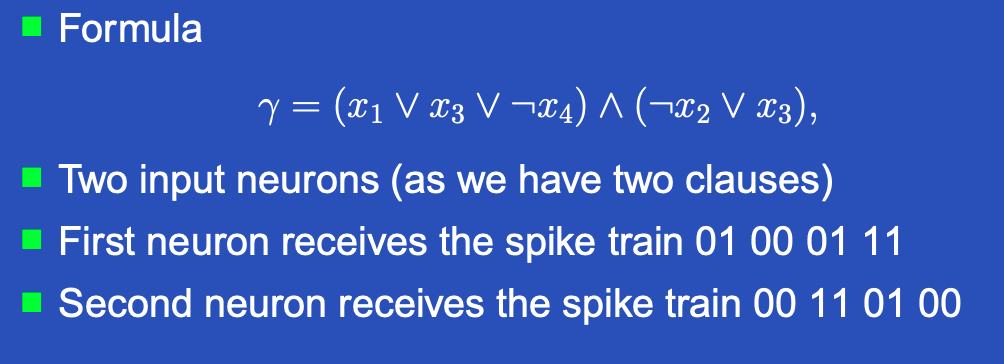
\includegraphics[width=0.8\linewidth]{img/sn p sol 1}
	\caption{Esempio di input per SN P (tramite spike train) di un'istanza del problema SAT.}
	\label{sn p sol 1}
\end{figure}
Vediamo ora com'è realizzata la struttura per risolvere un'istanza:
\begin{itemize}
\item Si ha un modulo $X_{i}$ per ogni variabile $x_{i}$.
\item Lo stesso vale per le clausole: si ha un modulo $Y_{j}$ per ogni clausola $C_{j}$.
\item Ogni modulo $X_{i}$ è connesso ad ogni altro modulo $Y_{j}$ tramite le sinapsi.
\item Si ha quindi un collegamento, sempre tramite sinapsi, da ogni clausola $Y_{j}$ ad un neurone che rappresenta l'output (vedi figura \ref{sn p sol 2}); quindi, se tutte le clausole $Y_{j}$ comunicano a questo neurone di essere soddisfatte, allora il neurone effettua uno spike (ossia la formula è soddisfacibile), altrimenti no (la formula non è soddisfacibile).
\end{itemize}

\paragraph{Conclusions}
as we have seen in the solution for SAT, to have an efficient solution for an NP-complete, or harder, problem we need to introduce feature with enhanced efficiency, such as the pre-computation we did with the relation between variable and clauses: \ref{Relation Between Variables And Clauses}.

\begin{figure}[h]
	\centering
	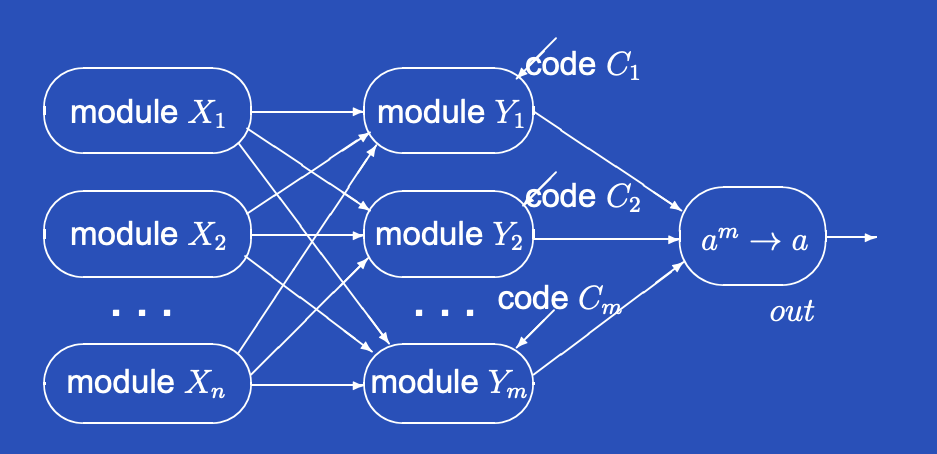
\includegraphics[width=0.8\linewidth]{img/sn p sol 2}
	\caption{Rappresentazione del sistema che risolve SAT tramite soluzione uniforme.}
	\label{sn p sol 2}
\end{figure}

\chapter{Genetic Algorithms}
\paragraph{Introduction}
there are some optimization problems that are not suited for classical algorithms, to those problems we can apply genetics algorithms to find a solution that is pretty close to the optimal one; some of those problems are:
\begin{itemize}
\item Unknown objective function.
\item Stochastic objective function.
\item Highly non linear objective function.
\end{itemize}
note that for every one of these type of problems, it may be necessary to use a different approach.

\paragraph{Main idea}
l'idea degli algoritmi genetici è la seguente: avere una popolazione di possibili soluzioni per un problema, quindi avere un metodo che permetta di ottenere una soluzione finale che si avvicini il più possibile ad una soluzione adeguata per il problema dato, possibilmente anche con un tempo accettabile.

\paragraph{General scheme}
\begin{enumerate}
\item Definizione della popolazione iniziale.
\item Ad ogni iterazione: selezionare alcuni individui dalla popolazione attuale.
\item Generare i nuovi individui: effettuare incroci e mutazioni a partire dagli individui selezionati al punto precedente.
\item Costruire la nuova popolazione: sostituire alcuni soggetti della popolazione attuale con quelli selezionati al punto precedente.
\item Fermarsi quando si è raggiunta una soglia di errore soddisfacente.
\end{enumerate}

\paragraph{Considerazioni}
faremo ora alcune considerazioni sui vari aspetti degli algoritmi genetici.

\subparagraph{Objective function}
how to quantify the quality of a solution? this is already a different task, because as we have seen we may not have an objective function, so it is mandatory to first understand how and why a solution is better than another one.

\subparagraph{Starting population}
how many individuals should an optimal population include? (the more the slower will be a single step of computation, but fewer steps will be required, the less, obviously the opposite, more steps required, but every steps will require less time).

\subparagraph{\% of population kept}
how many individuals should be kept from a step to the next one?

\subparagraph{Cross parents}
how should the crossing between individuals be done?

\subparagraph{Mutation}
how much mutation should be introduced? in general is good to have a low probability to introduce mutation (cause otherwise you may get to the optimum but then introduce the mutation and step away from it), but it is recommended to have it to enhance the possibility to escape a local optimum.

\subparagraph{Stop criteria}
gli algoritmi genetici, generalmente, terminano  in due condizioni: dopo un certo tempo, oppure quando si è raggiunta una certa soglia di errore.

\chapter{Social \& Swarm Algorithms}
\paragraph{Introduction} For social we mean a big set of very simple entities able to perform simple tasks, able to produce as a whole, a behaviour that allows to obtain  a general result; the group continuously share information between each other. There are two ways of share informations: met another entities and give them the information, or leave an information somewhere so that other entities can get it.

\paragraph{Very Simple Rules}
Very simple means: random rules or stochastic rules; random rules are good for two reason:
\begin{enumerate}
\item \textbf{Explore the whole space} if we have a big enough population, than the algorithm may be able to explore the whole space, not falling into local optimums.
\item \textbf{Escape local optimum} even if the population fall in a local optimum, then, if the random part weight enough, than the population will be able to escape the local optimum.
\end{enumerate}

\paragraph{No Central Control}
Every individual is evolving independently during the computation, so the only thing controlling the situation are the simple rules; these simple rules, even without a central control, are able to obtain an emergent behaviour of the whole population.

\paragraph{Other considerations}
let's now consider some pros and cons of social algorithms:
\subparagraph{Pros}
\begin{itemize}
\item Typically able to find the global optimum.
\item Wide range of problems: because the algorithm are not so specific, are able to solve a lot of problem having a lot of similar features between them.
\item Exploration / exploitation balance managing.
\end{itemize}

\subparagraph{Cons}
\begin{itemize}
\item Time required: maybe you already are on an optimum, but because the population doesn't know the whole space, the algorithm need to do some iterations before stop.
\item No exact repetition: because there are a lot of choices and random parts in the algorithm.
\item Consistency: cause you'll never know if the returned solution is actually the best.
\end{itemize}

\section{Ant Colony Optimization}
Ant colony optimization (ACO) is the first social algorithms, initially used to find a solution for travelling salesman problem; the idea is that an ant colony will try to find the shortest way between a food source and the nest; even with an obstacle, the ants will be able, after some time, to find a really good path between the two points; Ants are able to do this with the help of a pheromone that work in this way: it is released from every ant, but evaporate overtime, so, the more an ant follow a specific path, the higher will be pheromone level; this translate in the fact that ant following an actual shortest path will be faster that and ant following a longer, path, so, because the first ant will be faster,the ant will also be able to release more pheromone on the path; when a new ant get to a road junction, the it will decides to got to one way or the other according to some probability, not only checking the pheromone levels; For example, in most studies, the probability $P_{ij}$ of choose a route from node $i$ to node $j$ can be calculated by
$$
	p_{ij} = \dfrac{ \phi_{ij}^{\alpha} d_{ij}^{\beta} }{\displaystyle\sum_{i, j}^{n} \phi_{ij}^{\alpha} d_{ij}^{\beta} }
$$
where $a, b > 0$ are the so-called influence parameters, and $\phi_{ij}$ is the pheromone concentration on the route between $i$ and $j$. In addition, $d_{ij}$ is the desirability of the route (for example, the distance of the overall path). In the simplest case when $a = b = 1$, the choice probability is simply proportional to the pheromone concentration.

\paragraph{Other Parameters}
Other Parameters to think abut are the ones that may and should change during a computation, for example, in ACO there are two parameters: the deposition and the decay of the pheromone; in the literature an incremental deposition and exponential decay are typically used.

\paragraph{Stop Criteria}
There are different possible choices also considering the stop criteria, in fact: 1) One could be, as usual, to stop after a certain number of iterations 2) Another one may involve the best solution so far: considering the last and second to last solution, if the two are wide apart then it may be probable that another iteration may still increase the quality of the solution; otherwise, if the two are already pretty close, it is possible that we are already close to the optimum and so there's no sense in following along the computation.

\section{Particle Swarm Optimization}
\paragraph{Introduction} Particle Swarm Optimization (PSO) è un algoritmo sociale basato sugli stormi di uccelli che cercano cibo, da ciò deriva il nome. L'idea di questa tecnica applicata a graph drawing è che ogni particella non rappresenta un vertice, ma bensì una configurazione del grafo, ossia una possibile soluzione; Alcuni vantaggi di PSO sono i seguenti: 1) è altamente parallelizzabile 2) non usa il gradiente 3) utilizza pochi hyperparameters. Vediamo ora più nello specifico i parametri di un particella $P_i$, all'istante $t$:
$$P_i^{t} = [ x_{0, i}^{t}, x_{1, i}^{t}, x_{2, i}^{t}, ... ,x_{n, i}^{t},] $$
dove le varie $x_{i, j}^{t},$ sono le coordinate rispetto allo spazio, della particella i-esima all'istante di tempo $t$; si noti che è difficile trovare il giusto \textbf{equilibrio} tra numero di elementi e tempo di esecuzione, infatti, se si hanno troppi elementi, non solo si avrà un tempo di simulazione più alto del necessario, ma si incapperà nella situazione in cui si avranno alcune particelle sovrapposte (sulla stessa posizione) ed è quindi una situazione non ottimale. Oltre alle coordinate nello spazio, ad ogni particella è associata una velocità in un determinato istante di tempo $t$:
$$ V_{i}^{t} = [v_{0,i}^{t}, v_{1,i}^{t}, v_{2,i}^{t}, ... , v_{n,i}^{t}] $$
questa velocità indica il movimento della particella di riferimento in una data direzione; conoscendo quindi l'attuale posizione della particella ($P_i^{t}$) possiamo calcolare la successiva velocità: ($V_{i}^{t+1}$), quindi, una volta calcolata la velocità successiva, possiamo calcolare la posizione successiva della particella:
$$ P_{i}^{t+1} =  P_{i}^{t} + V_{i}^{t+1}$$
dove
$$V_{i}^{t+1} = w V_{i}^{t} + c_1 r_1(P_{PB, i}^{t} - P_{i}^{t}) + c_2 r_2 (P_{GB}^{t} - P_{i}^{t})$$
con:
\begin{itemize}
\item $w V_{i}^{t}$ parametro che serve come sorta di inerzia che permette di modificare la velocità solo in un certo range; questa scelta di implementazione rende l'algoritmo più simile al comportamento degli uccelli veri, infatti, un uccello che ha visto un pezzo di cibo nel punto $A$, e quindi inizia ad avvicinarsi ad esso, se dopo alcuni istanti di tempo si accorge che c'è un altro pezzo di cibo nel punto $B$, allora esso non cambierà direzione in un istante, ma ci metterà almeno qualche istante.
\item $c_1 r_1(P_{PB, i}^{t} - P_{i}^{t})$ questa è la personal knowledge, ossia ciò che conosce la particella.
\item $c_2 r_2 (P_{GB}^{t} - P_{i}^{t})$ questa è la global knowledge, ossia il pensiero comune del gruppo.
\end{itemize}
Facciamo ora delle considerazioni sui valori assunti dai parametri:
\begin{itemize}
\item $r_1 \in [0, 2]$ è ciò che pensa la particella, all'inizio assume un valore random.
\item $r_2 \in [0, 2]$ è ciò che pensa il gruppo, all'inizio assume un valore random.
\item $w$ tipicamente $\simeq 0,72$.
\item $c_1$ tipicamente $\simeq 2,05$ da notare che è un valore simile a $r_1$.
\item $c_2$ tipicamente $\simeq 2,05$ da notare che è un valore simile a $r_2$.
\item tipicamente si cerca di ottenere che $c_1 + c_2 \geq 4$.
\end{itemize}

\paragraph{$c_1$ \& $c_2$ setup}
Ora possiamo discutere di un'altra opzione, ossia si può scegliere di tenere $c_1$ e $c_2$ statici, oppure si può scegliere di farli variare nel tempo; avere un valore più alto di $c_1$ rispetto a $c_2$ significa che si da valore al pensiero della particella e quindi si favorisce la fase di exploration, viceversa, si starà favorendo la fase di exploitation.

Quindi, un buon metodo per settare $c_1$ e $c_2$ è di iniziare con $c_1$ molto alto e $c_2$ molto basso, quindi, abbassare gradualmente $c_1$, e alzare gradualmente $c_2$, si noti che al termine non si dovrà avere $c_1 = 0$ e $c_2 = max$, altrimenti nessuno si avvicinerà più all'ottimo, è quindi importante che $c_1$ non sia mai pari a $0$.

\paragraph{Quando fermarsi?}
Alcuni criteri di arresto utilizzati sono i seguenti:
\begin{itemize}
\item L'algoritmo verrà arrestato se si è arrivati ad un tempo di esecuzione pari a circa $\vert V \vert$.
\item Si può anche scegliere di terminare dopo un certo numero di iterazioni.
\item O, ancora, si può scegliere di terminare nel momento in cui si nota che la soluzioni attuale non migliora di molto rispetto alle precedenti iterazioni.
\end{itemize}

 (nel caso specifico di graph drawing, una volta che la procedura è terminata, si deve scegliere la particella migliore, confrontando le varie particelle tra loro).

\paragraph{Relazione tra PSO e graph drawing}
Quando vogliamo applicare PSO dobbiamo trovare un modo per mettere in relazione la descrizione di PSO con il problema graph drawing, ad esempio, considerando la seguente formula:
$$P_i^{t} = [ x_{0, i}^{t}, x_{1, i}^{t}, x_{2, i}^{t}, ... ,x_{n, i}^{t},] $$
avremo che ogni $x$ deve rappresentare uno specifico vertice, nello specifico, le coordinate di un vertice, si noti quindi che, a seconda della dimensionalità del disegno (2d, 3d, ecc...) ogni $x$ non sarà un singolo valore, ma una coppia, una tripla ecc...; il numero di particelle utilizzato in PSO per risolvere graph drawing è molto importante, si noti che esso dipende dalla \textbf{dimensione dello spazio}, non dalla dimensione del grafo.

Definiamo  ora la funzione obiettivo tramite le forze che abbiamo descritto in precedenza:
$$f(x) = \displaystyle\sum_{i,j \in E} f_a (i, j) + \displaystyle\sum_{i,j \in V} f_r (i, j)$$
Si noti che la forza attrattiva è applicata agli archi, invece la forza repulsiva è applicata a coppie di vertici; si può anche notare che vogliamo minimizzare il valore di questa funzione, ma allora perché sommiamo invece che sottrarre la seconda somma alla prima? lo facciamo in quanto la seconda somma avrà valore negativo, infatti il valore della forza repulsiva, per come lo abbiamo definito noi, è negativo.

\paragraph{Complessità}
La complessità di questa tecnica, considerato un numero di iterazioni pari a $i$ ed un numero di particelle pari a $m$, se $i, m \ll {\vert V \vert}^2 \Rightarrow T(n) = \bigcirc({\vert V \vert}^2)$, se vogliamo abbassare il tempo di questa tecnica, dobbiamo considerare Bernes-Hut!

\chapter{Cellular Ants Computing}

\paragraph{Introduction} In this section we describe some methods based on \textbf{ant colony optimization} and \textbf{cellular automata}; it want to be a new formalism based on the two, exploiting their main pros: ACO is able to find pretty good solutions, CA offer a strong parallelism.

\section{Data Clustering}
The data clustering problem is a known problem in which it is required to group data of the same type in different clusters.

\paragraph{Ant sleeping model}
one way researchers have tried to optimize the data clustering problem was by implementing the ant sleeping model; this model is based upon the fact that, once an ant feel safe, it can go to sleep; initially, ants are distributed on the space in a random way; then all ants will start to reach for a safer place, until satisfied, and so they go to sleep. In addition, when an ant at sleeping state is not satisfied with its current position, it becomes active and starts its exploration to find an additional “comfort” position. The feeling of safety is based upon the number of similar, with similar it is meant similar physique, ants between the considered ant and how much close are relatively to each others.

\paragraph{Ant swapping model}
The aforementioned method exploits a fraction of the ACO advantages disregarding basic principles that could be proven significantly beneficial in data clustering. A more relevant method with the concept of cellular ants includes multiple additions regarding the cell's states and the corresponding transition rules in order to exploit fully their advantages (Moere and Clayden 2005). The method abolishes the term of sleeping state for every cellular ant and considers that the actions of every agent are determined by the discrete number of similar ants in their neighbourhood. Two other factor implemented in this model: \textbf{(i)} the possibility to swap two ants to internally order a cluster \textbf{(ii)} defining more cell's states in order to represent ant's pheromone levels.

\section{Swarm Robotics}
In this section we will introduce the use of cellular ant computing in the problem of Swarm robotics. A cellular ant-based model, named as cellular automata, was introduced to define the pathway of a robot in an operating area depending on its final objective. The approach considers that the robots operate in a type of intelligent floor in order to comply with the stigmergy feature of ACO algorithms. The floor is divided into multiple Finite-State Machines (FSM) in order to develop a two- dimensional mesh whose nodes form tiles. Every FSM can be denoted with finite values similar to a classical CA. The model considers also values for the pheromone concentrations except the states that correspond to robots. Moreover, every FSM comprises both a transmitter and a receiver to simulate the communication that the robots must exhibit. Three scenarios as final tasks were tested: \textbf{(i)} parking, \textbf{(ii)} food-finding, and \textbf{(iii)} maze-threading.

\chapter{Unconventional Computational problems}
\paragraph{Introduction}
This section is dedicated to problems that necessarily require an unconventional approach and unconventional computation to be solved; this is because the various constraints, mathematical o timing, of the problems made it impossible for conventional computations to solve them; more in detail, some of those problems require an hardware that is not fixed: the number of processors will depend on the input dimension.

\begin{definizione}
\title{\emph{Unconventional computational problem}}

A computation requiring n algorithmic steps per time unit, where n is larger than 1. Such a computation cannot be performed successfully on a computer that can only perform a finite and fixed number m of algorithmic steps per time unit, where m is smaller than n.
\end{definizione}

\paragraph{Unconventional computational problem}
A computation requiring n algorithmic steps per time unit, where n is larger than 1. Such a computation cannot be performed successfully on a computer that can only perform a finite and fixed number m of algorithmic steps per time unit, where m is smaller than n.

\paragraph{Computations Obeying Mathematical Constraints}
There exists a family of computational problems where, given a mathematical object satisfying a certain property, we are asked to transform this object into another which also satisfies the same property. Furthermore, the property is to be maintained throughout the transformation, and be satisfied by every intermediate object, if any. More generally, the computations we consider here are such that every step of the computation must obey a certain predefined mathematical constraint. (Analogies from popular culture include picking up sticks from a heap one by one without moving the other sticks, drawing a geometric figure without lifting the pencil, and so on.) An example of computations obeying a mathematical constraint is provided by a variant to the problem of sorting a sequence of numbers stored in the memory of a computer. For a positive even integer $n$, where $n \geq 8$, let $n$ distinct integers be stored in an array $A$ with $n$ locations $A[1], A[2], . . . , A[n]$, one integer per location. Thus $A[j]$, for all $1 \leq j \leq n$, represents the integer currently stored in the \textit{j}th location of $A$. It is required to sort the $n$ integers in place into increasing order, such that:
\begin{enumerate}
\item After step $i$ of the sorting algorithm, for all $i \geq 1$, no three consecutive integers satisfy
\begin{equation}
A[j] > A[j+1] > A[j+2]
\end{equation}
for all $1 \leq j \leq n - 2$.
\item When the sort terminates we have
\begin{equation}
A[1] < A[2] < ... < A[n]
\end{equation}
\end{enumerate}
This is the standard sorting problem in computer science, but with a twist. In it, the journey is more important than the destination. While it is true that we are interested in the outcome of the computation (namely, the sorted array, this being the destination), in this particular variant we are more concerned with how the result is obtained (namely, there is a condition that must be satisfied throughout all steps of the algorithm, this being the journey). It is worth emphasizing here that the condition to be satisfied is germane to the problem itself; specifically, there are no restrictions what- soever on the model of computation or the algorithm to be used. Our task is to find an algorithm for a chosen model of computation that solves the problem exactly as posed. One should also observe that computer science is replete with problems with an inherent condition on how the solution is to be obtained. Examples of such problems include inverting a nonsingular matrix with- out ever dividing by zero, finding a shortest path in a graph without examining an edge more than once, sorting a sequence of numbers without reversing the order of equal inputs (stable sorting), and so on.

\paragraph{Time-Varying Computational Complexity}
Here, the computational complexity of the problems at hand depends on time (rather than being, as usual, a function of the problem size). Thus, for example, tracking a moving object (such as a spaceship racing toward Mars) becomes harder as it travels away from the observer.
Suppose that a certain computation requires that $n$ independent functions, each of one variable, namely, $f_1(x_1), f_2(x_2), ..., f_n(x_n)$, be computed. Computing $f_i(x_i)$ at time $t$ requires $C(t) = 2^t$ algorithmic steps,for $t\geq 0$ and $1 \leq i \leq n$. Further, there is a strict deadline for reporting the results of the computations: All $n$ values $f_1(x_1), f_2(x_2), ..., f_n(x_n)$ must be returned by the end of the third time unit, that is, when $t = 3$.
It should be easy to verify that no sequential computer, capable of exactly one algorithmic step per time unit, can perform this computation for $n = 3$. Indeed, $f_1(x_1)$ takes $C(0) = 2^0 = 1$ time unit, $f_2(x_2)$ takes another $C(1) = 2^1 = 2$ time units, by which time three time units would have elapsed. At this point none of $f_3(x_3), ..., f_n(x_n)$ would have been computed. By contrast, an $n$-processor parallel computer solves the problem handily. With all processors operating simultaneously, processor $i$ computes $f_i(x_i)$ at time $t = 0$, for $1 \leq i \leq n$. This consumes one time unit, and the deadline is met.

\paragraph{Time-Varying Variables}
For a positive integer $n$ larger than 1, we are given $n$ functions, each of one variable, namely, $f_1, f_2, f_n$, operating on the $n$ physical variables $x_1, x_2, ..., x_n$, respectively. Specifically, it is required to compute $f_i(x_i)$ for $i = 0 1, 2, .., n$. For example, $f_i(x_i)$ may be equal to $x_i^2$. What is unconventional about this computation is the fact that the $x_i$ are themselves (unknown) functions $x_1(t), x_2(t), ..., x_n(t)$ of the time variable $t$. It takes one time unit to evaluate $f_i(x_i(t))$. The problem calls for computing $f_i(x_i(t))$, $1 \leq i \leq n$, at time $t = t_0$. Because the function $x_i(t)$ is unknown, it cannot be inverted, and for $k > 0$, $x_i(t_0)$ cannot be recovered from $x_i(t_0 + k)$. Note that the value of an input variable $x_1(t)$ changes at the same speed as the processor in charge of evaluating the function $f_i(x_i(t))$.
A sequential computer fails to compute all the $f_i$ as desired. Indeed, suppose that $x_1(t_0)$ is initially operated upon. By the time $f_i(x_i(t_0))$ is computed, one time unit would have passed. At this point, the values of the $n - 1$ remaining variables would have changed. The same problem occurs if the sequential computer attempts to first read all the $x_i$, one by one, and store them before calculating the $f_i$.
By contrast, a parallel computer consisting of $n$ independent processors may perform all the computations at once: For $1 \leq i \leq n$, and all processors working at the same time, processor $i$ computes $f_i(x_i(t_0))$, leading to a successful computation.

\paragraph{Interacting Variables}

\paragraph{The Global Variable Paradigm}

\part{Quantum Computing}

\section{Introduction}

\paragraph{Introduction}
Able, with reverse computation, to produce increasingly less waste heat (see Landauer's principle).

Computational power of quantum computer: this subject is not clear, in fact in theory QPU are more powerful than CPU, from the computational point of view, there is only one thing that  QPU are able to do: to generate perfectly random numbers.

\paragraph{Quantum Advantage / Supremacy}
it is a probabilistic quantum algorithm

\paragraph{Scalability}
One of the main problems when realizing quantum computers is scalability, in fact, increasing the number of bits is really difficult; for this reason, companies often speaks about quantum volume instead of qubit.
Scalability is a problem because, \hl{most} algorithms "use" logic qubit; several physical qubit are needed to implement one single theoretical/logic qubit, because of the noise and other problems. For example, if a theoretic algorithm say it need 100 logical qubit it means that the quantum computer, to be able to implement those 100 logical qubit, it needs $100$ (logical qubit) $*$ $10000$ (physical qubit).

\paragraph{Quantum Experiment}
See page 10 of the textbook; photons model: unit vector where unit means $||\overrightarrow{\alpha}|| = 1$, instead of this notation we will use the bra-ket notation because it is more clear and easier to understand when performing a lot of calculations.
\paragraph{bra-ket notation}
$ \langle v |$ is called the "bra" of $v$; $| v \rangle $ is called the "ket" of $v$; to perform the inner product of the two we just write $ \langle v | v \rangle $.

We have that $| v \rangle = a | \rightarrow \rangle + b | \uparrow \rangle $ and, when both the coefficients $a, b$ are non-zero, then $ a | \rightarrow \rangle + b | \uparrow \rangle $ is called a \textit{superposition} of $| \uparrow \rangle $ and $| \rightarrow \rangle $

\pagebreak
\section{Single-Qubit Systems}
\subsection{Physical Representations Of Qubits}
\begin{itemize}
\item Polarized Photons
\item Energy Levels of electrons
\item Spin of particles (up or down)
\item Creation / annihilation
\end{itemize}

\subsection{Mathematical Representation Of Qubits}
From a mathematical point of view, qubits are two-dimensional complex vector spaces (also called "Hilbert space") implemented as a two-state quantum systems, where the two states are typically called ground / base states ($ |0\rangle $, $ |1\rangle $).

Even if there are only two base states, a qubit can assume an infinite number of possible states (that are not ground states), those states are linear combination of ground state: 

\begin{itemize}
\item Standard bases: $ \lbrace |0\rangle, |1\rangle \rbrace $
\item $ |v\rangle = a|0\rangle + b|1\rangle \in \mathbb{C}^{2} $ with $a, b \in \mathbb{C} $ such that $ |a|^{2} + |b|^{2} = 1 $ and with $ |v\rangle $ of unit length, and so we can also write it as $ \langle v | v \rangle = 1 $.
\item Other bases:
\begin{itemize}
\item Photons polarizations: first base $ |\uparrow \rangle $, $ \vert \rightarrow \rangle $; second base $ |\nearrow \rangle $, $ \vert \nwarrow \rangle $.
\item Spin up $ |\uparrow\rangle $ or spin down $ |\downarrow\rangle $.
\end{itemize}
\end{itemize} 
Let $V$ be a complex space whose elements are vector of complex numbers, then the inner product (dot product) is the following function
$$ \langle \cdot | \cdot \rangle : V \times X \rightarrow \mathbb{R}^{+}_{0} $$
with the following properties:
\begin{enumerate}
\item Inner product: $ \langle v | v \rangle \in \mathbb{R}^{+}_{0} $ and is typically 1.
\item $ \langle v_2 | v_1 \rangle = \overline{\langle v_1 | v_2 \rangle}$ where $\overline{z} = a-ib$ and $z = a+ib$
\item Linearity:
$$ ( a  \langle v_2 | + b \langle v_3 | ) \quad | v_1 \rangle =
a  \langle v_2 | v_1 \rangle + b \langle v_3 | v_1 \rangle $$
\item Orthogonality: $ v_1 \perp v_2 $ if and only if $ \langle v_1 | v_2 \rangle = 0 $
\item Length (norm) of a vector $ | v \rangle $ represented as
$ | | v \rangle | = \sqrt{ \langle v | v \rangle }$
\item Example considering
$|0\rangle =
\begin{bmatrix}
1 \\
0 \\
\end{bmatrix}$
$ |1\rangle =
\begin{bmatrix}
0 \\
1 \\
\end{bmatrix}
$
so we have that

\begin{align*}
    |v\rangle &= a|0\rangle + b|1\rangle \\
    &= a \begin{bmatrix}
0 \\
1 \\
\end{bmatrix}
+
b
\begin{bmatrix}
1 \\
0 \\
\end{bmatrix} \\
&= \begin{bmatrix}
a \\
b \\
\end{bmatrix}
\end{align*}
\item Note: there may be some relationships between representations in different bases, considering the photon polarizations we have two bases and this relation holds between them:
\begin{itemize}
\item $ |\nearrow\rangle = \dfrac{1}{\sqrt{2}} |\uparrow\rangle + \dfrac{1}{\sqrt{2}} |\rightarrow\rangle $
\item $ |\rightarrow\rangle = \dfrac{1}{\sqrt{2}} |\nearrow\rangle - \dfrac{1}{\sqrt{2}} |\nwarrow\rangle $
\item $ |\nwarrow\rangle = \dfrac{1}{\sqrt{2}} |\uparrow\rangle - \dfrac{1}{\sqrt{2}} |\rightarrow\rangle $
\item $ |\uparrow\rangle = \dfrac{1}{\sqrt{2}} |\nearrow\rangle + \dfrac{1}{\sqrt{2}} |\nwarrow\rangle $
\end{itemize}
\end{enumerate}

\subsection{See page 15 of the book}

\subsection{Example Of Bra Ket}
Considering
$|0\rangle =
\begin{bmatrix}
1 \\
0 \\
\end{bmatrix}$
$ |1\rangle =
\begin{bmatrix}
0 \\
1 \\
\end{bmatrix}
$
we have that, because $0$ and $1$ are real numbers, they do not have an imaginary component, so, the complex conjugate of a real number remain the number itself, and so
$ \langle0| = (1 \quad 0) $ and $ \langle1| = (0 \quad 1) $
so, the bra ket of $0$ with itself $ \langle  0 | 0 \rangle $ is the following inner product: $$ \langle  0 | 0 \rangle  = (1 \quad 0) * \begin{bmatrix} 1 \\ 0 \ \end{bmatrix} = 1*1 + 0*0 = 1 $$
the exact same happen considering $ \langle 1|1 \rangle $; if we now consider $ \langle 1|0 \rangle $ or $ \langle 0|1 \rangle $, they both have $0$ as result, because they are orthogonal, in fact, $ |0\rangle $ and $|1\rangle$ are orthonormal bases.

\paragraph{Filtering}
To filter out the first or second component of a vector we can respectively use the bra of $0$ or the bra of $1$, considering
$$
| v \rangle = a | 0 \rangle + b | 1 \rangle =
\begin{bmatrix}
a \\
b \\
\end{bmatrix}
$$
we can use the bra of $0$ to filter out the first component:
$$
\langle 0 | v \rangle
=
(1 \quad 0)
\begin{bmatrix}
a \\
b \\
\end{bmatrix}
=
a
$$
and, of course, we can use the bra of $1$ to filter out the second component:
$$
\langle 1 | v \rangle
=
(0 \quad 1)
\begin{bmatrix}
a \\
b \\
\end{bmatrix}
=
b
$$

\paragraph{Conjugate Component}
We can now consider the bra of $v$ instead of the ket of $v$; in general, the result will be a complex conjugate;
$$
\langle v | 0 \rangle
=
(\overline{a} \quad \overline{b})
\begin{bmatrix}
1 \\
0 \\
\end{bmatrix}
=
\overline{a}
$$

$$
\langle v | 1 \rangle
=
(\overline{a} \quad \overline{b})
\begin{bmatrix}
0 \\
1 \\
\end{bmatrix}
=
\overline{b}
$$

\subsection{Single-Qubit Measurement}
Quantum theory postulates that any device that measure a two-state quantum system \textbf{must} have two states whose representative vectors $ \vert u \rangle $ or $ \vert u^{\perp} \rangle $, form an \textbf{orthonormal basis} for the associated vector space.
For example, if we consider a measurement device such as one for measuring the polarization of photons with two associated bases
$ \lbrace \vert u \rangle, \vert u^{\perp} \rangle \rbrace $
then we are able to measure a state
$ \vert v \rangle = a \vert u \rangle + b \vert u^{\perp \rangle} $
the measure of the sate
$ \vert v \rangle $
will give:
\begin{itemize}
\item $ \vert u \rangle $ with probability $ \vert a^{2} \vert $
\item $ \vert u^{\bot} \rangle $ with probability $ \vert b^{2} \vert $
\end{itemize}
This behaviour of measurement is an axiom of quantum mechanics, It is not derivable from other physical principles; rather, it is derive from the empirical observation of experiment with measuring devices. Usually, if we say "measure a qubit" without further elaboration, we mean that the measurement is with respect to the standard basis
$ \lbrace | 0 \rangle, | 1 \rangle \rbrace $.

Measurement of a quantum state change the state. If a state
$ \vert v \rangle = a \vert u \rangle + b \vert u^{\perp \rangle} $
is measured as
$ \vert u \rangle $
then the state
$ \vert v \rangle $
changes to 
$ \vert u \rangle $.

While the mathematics of measuring a qubit in the superposition state
$ a \vert 0 \rangle + b \vert 1 \rangle $
with respect to the standard bases is clear, measurement brings up the questions as to the meaning of a superposition. To begin with, the notion of superposition is bases dependent; all states are superposition with respect to some bases and not with respect to others. For instance,
$ a \vert 0 \rangle + b \vert 1 \rangle $
is a  superposition with respect to the bases
$ \lbrace | 0 \rangle, | 1 \rangle \rbrace $
but is not with respect to
$ \lbrace a \vert 0 \rangle + b \vert 1 \rangle, \overline{b} \vert 0 \rangle + \overline{a} \vert 1 \rangle \rbrace $.

Given that that qubits can take on any one of infinitely many states, one might hope that a single qubit could store lots of classical information. However, the properties of quantum measurement severely restrict the amount of information that can be extracted from a qubit. Information about a quantum bit can be only obtained by measurement, and any measurement results in one of only two states, the two basis states associated with the measuring device; \textbf{thus, a single measurement yields at most a single classical bit of information}.

It is also not possible to measure a qubit's state in two ways, even indirectly by coping the qubit's state and measuring the copy (\hl{see section about no-cloning principle}).

\subsection{A Quantum Key Distribution Protocol - BB84}
\paragraph{Introduction}
Considering the Diffie-Hellman protocol, we know that while it remains secure against all known classical attacks, the problem on which it is based, the discrete logarithm, is tractable on a quantum computer ( \hl{see section on Shor's algorithm for the discrete logarithm problem}). So, if real quantum computer will ever be built, the discrete logarithm problem will be tractable; this means that we need a way to substitute Diffie-Hellman, one way could be the BB84 protocol.

\paragraph{BB84}
The earliest quantum key distribution protocol is known as BB84, it is as follow: Alice and Bob are connected by two public channels: an ordinary bidirectional classical channel and a unidirectional quantum channel. The quantum channel allowa Alice to send a sequence of single qubits to Bob. Both channels can be observed by an eavesdropper Eve. This situation in illustrated in figure \ref{BB84}.

\begin{figure}[h]
	\centering
	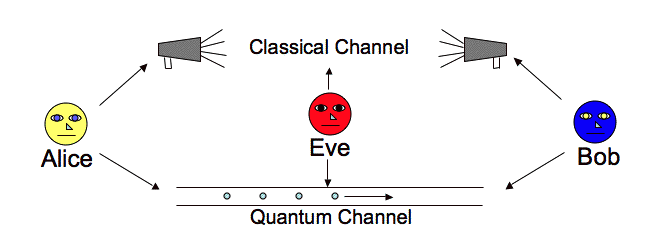
\includegraphics[width=0.7\linewidth]{img/BB84}
	\caption{Alice and Bob wish to agree on a common key not know to Eve.}
	\label{BB84}
\end{figure}

To begin the process of establishing a private key, Alice uses quantum or classical means to generate a random sequence of classical bit values. As we will see, a random subset of this sequence will be the final private key. Alice then randomly encodes each bit of this sequence in the polarization state of a photon by randomly choosing for each bit one of the following to agreed-upon bases in which to encode it: the standard basis or the Hadamard basis. She sends this sequence of photons to Bob through the quantum channel.

Bob measures the state of each photon he receives by randomly picking either basis. Over the classical channel, Alice and Bob check that Bob has received a photon for every one Alice has sent, and only then do Alice and Bob tell each other the bases they used for encoding and decoding each bit. When the choice of bases agree, Bob's measured bit value agrees with the bit value that Alice sent. When they chose different bases, the chance that Bob's bit matches Alice's is only 50 percent. Without revealing the bit value themselves, which would also reveal the value to Eve, there is no way for Alice and Bob to figure out which of these bit values agree and which do not. So they simply discard all the bits on which their choice of bases differed. An average of 50 percent of all bits transmitted remain. Then, depending on the level of assurance they require, Alice and Bob compare a certain number of bit values to check that no eavesdropping has occurred. These bits will also be discarded, and only the remaining bits will be used as their private key.

\paragraph{Notes On The Protocol}
Since Alice, during the transmission of the qubits, has not told yet Bob her sequence of bases, Eve does not know in which basis to measure each bit. If she randomly measure the bits, she will measure using the wrong basis approximately half of the time. When she user the wrong basis to measure, the measurement changes the polarization of the photon before it is resent to Bob.This change in the polarization means that, even if Bob measure the photon in the same basis as Alice used to encode the bit, he will get the correct bit value only half the time. So, the fact that someone is eavesdropping can be detected by Alice and Bob.

The security of this protocol, like other pure key distribution protocol such as Diffie-Hellman, is vulnerable to a \textit{man-in-the-middle} attack in which Eve impersonates Bob to Alice and impersonates Alice to Bob. To guard against such an attack, Alice and Bob need to combine it with an authentication protocol, be it recognizing each other's voice or more mathematical authentication protocol.

\subsection{The State Space of a Single-Qubit System}
The \textit{state space} of a classical or quantum physical system is the set of all possible states of the system. Depending on which properties f the system are under consideration, a state of the system consist of any combination of the positions, momenta, polarizations, spins, energy, and so on pf the particle in the system. When we are considering only polarization states of single photon, the state space is all possible polarizations. \textbf{More generally, the state space for a single qubit, no matter how it is realized, is the set of all possible qubits values},
$ \lbrace a \vert 0 \rangle + b \vert 1 \rangle \rbrace $
where
$ \vert a^{2} \vert + \vert b^{2} \vert = 1 $
and
$ a \vert 0 \rangle + b \vert 1 \rangle $
and
$ a' \vert 0 \rangle + b' \vert 1 \rangle $
are considered the same qubit if there exist a complex number $c$ such that $ \vert c \vert = 1 $ and
$ a \vert 0 \rangle + b \vert 1 \rangle = c ( a' \vert 0 \rangle + b' \vert 1 \rangle ) $.

\subsubsection{Relative Phases versus Global Phases}
The multiple by which two vectors representing the same quantum state differ is called the \textit{global phase} and has no physical meaning. We use the equivalence relation
$ \vert v \rangle \sim \vert v' \rangle $
to indicate that 
$ \vert v \rangle = c \vert v' \rangle $
for some complex global phase
$ c = e^{\textbf{i}\phi} $

A physical important quantity is the relative phase of a single-qubit state
$ a \vert 0 \rangle + b \vert 1 \rangle $.
The relative phase (in the standard basis) of a superposition
$ a \vert 0 \rangle + b \vert 1 \rangle $
is a measure of the angle in the complex plane between the two complex numbers $a$ and $b$.
More precisely, the relative phase is the modulus one complex number
$ e^{\textbf{i} \phi } $
satisfying
$ \dfrac{a}{b} = e^{\textbf{i} \phi } \dfrac{ \vert a \vert }{ \vert b \vert } $.
Two superposition
$ a \vert 0 \rangle + b \vert 1 \rangle $
and
$ a' \vert 0 \rangle + b' \vert 1 \rangle $
whose amplitudes have the same magnitudes but that differ in a relative phase represent different states.

\textbf{The physical meaningful relative phase and physical meaningless global phase should not be confused.}

\subsubsection{Geometric Views of the State Space of a Single Qubit}

\paragraph{Bloch Sphere}
The bloch sphere is a famous and important representation for the quantum state of a single qubit. In this representation there is a one-to-one correspondence between single-qubit states and points in the space (that is the surface of the sphere). Considering the superposition
$ a \vert 0 \rangle + b \vert 1 \rangle $
if we do some multiplication, we can say that $a$ is real and greater than $0$, this is the reason why we can map each state, represented by the complex number
$ \alpha = s + \textbf{i} t $
onto the unit sphere in three real dimensions. Considering the point $ (s, t) $ it is mapped to the point of the sphere as follow:
$$
(s, t)
\mapsto
\left(
\dfrac{ 2s }{ { \vert \alpha \vert }^{2} + 1 },
\dfrac{ 2t }{ { \vert \alpha \vert }^{2} + 1 },
\dfrac{ 1 - { \vert \alpha \vert }^{2} }{ { \vert \alpha \vert }^{2} + 1 }
\right)
$$

\begin{figure}[h]
	\centering
	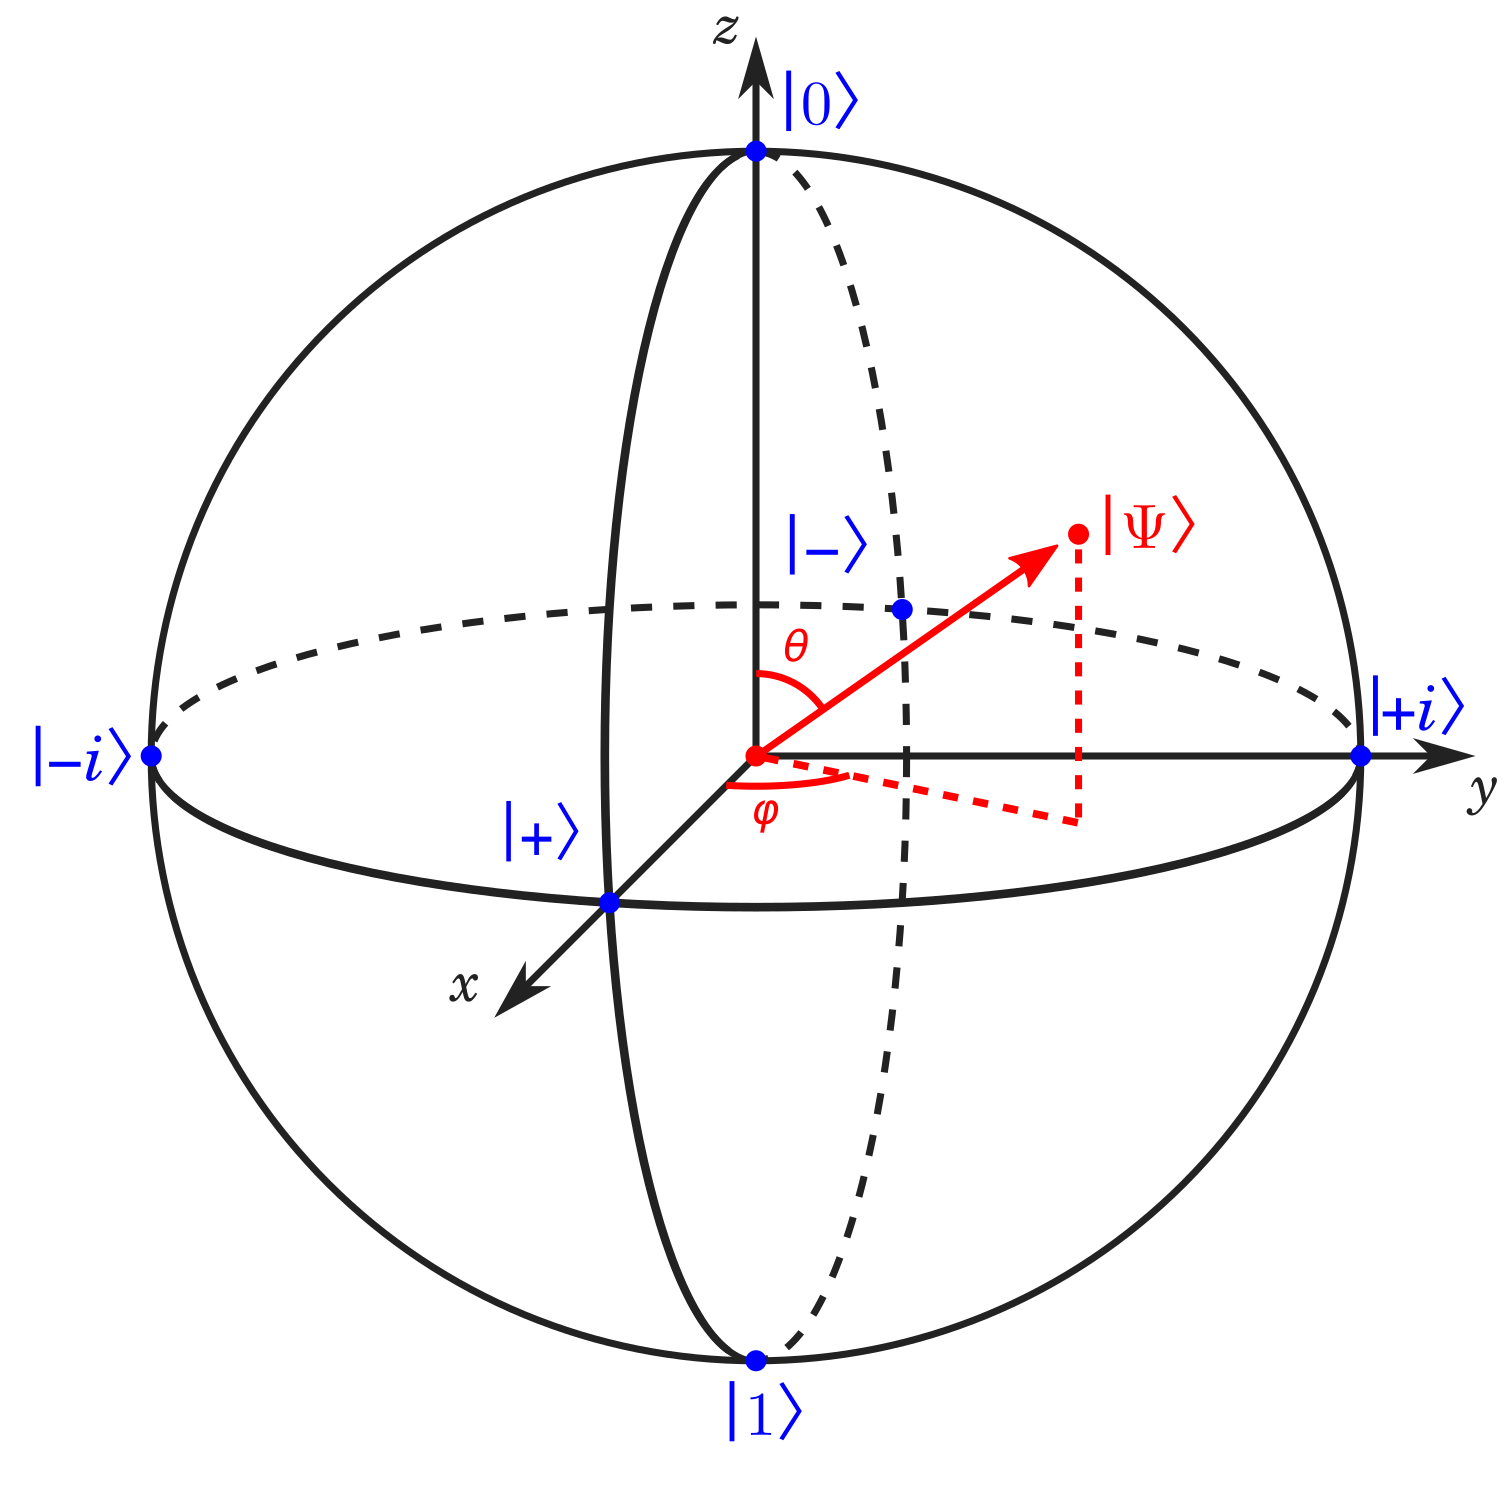
\includegraphics[width=0.6\linewidth]{img/bloch sphere}
	\caption{Representation of the bloch sphere.}
	\label{Bloch sphere}
\end{figure}

Note that vectors at opposite side of the sphere form an orthonormal basis. It is also possible to represent points on the sphere using two planes of the bloch sphere: the horizontal and the vertical plane.

\pagebreak
\section{Multiple-Qubit Systems}
There a big difference in how the size of a system grows:
\begin{itemize}
\item The size of a multiple-qubit system grows exponentially.
\item The size of a classical system grows linearly.
\end{itemize}


\pagebreak
\section{Exam's notes}

\begin{itemize}
\item Know how to "handle" circuits.
\item Know the algorithm seen.
\end{itemize}

\section{Temporaries}

\begin{itemize}
\item $a
\begin{bmatrix}
0 \\
1 \\
\end{bmatrix}
+
b
\begin{bmatrix}
1 \\
0 \\
\end{bmatrix}
=
\begin{bmatrix}
a \\
b \\
\end{bmatrix}
$

\item
$
H = \dfrac{1}{\sqrt{2}}
\begin{bmatrix}
1 & 1 \\
1 & -1 \\
\end{bmatrix}
$
\begin{itemize}
\item $ H \cdot \vert 0 \rangle =
\begin{bmatrix}
1 & 1 \\
1 & -1 \\
\end{bmatrix}
\cdot
\begin{bmatrix}
1 \\
0 \\
\end{bmatrix}
=
\begin{bmatrix}
1 \\
1 \\
\end{bmatrix}
$
\item $ H \cdot \vert 1 \rangle =
\begin{bmatrix}
1 & 1 \\
1 & -1 \\
\end{bmatrix}
\cdot
\begin{bmatrix}
0 \\
1 \\
\end{bmatrix}
=
\begin{bmatrix}
1 \\
-1 \\
\end{bmatrix}
$
\end{itemize}
\end{itemize}

\end{document}
